%%%%%%%%%%%%%%%%%%%%%%%%%%%%%%%%%%%%%%%%%%%%%%%%%%%%%%%%%%%%%%%%%%%%%%%%%%%%%%%
%% LaTeX-Vorlage für Abschlussarbeiten                                       %%
%% (TH Köln -Campus Gummersbach, Fak. 10)                                    %%
%%                                                                           %%
%% Gemäß dem Merkblatt zur Anfertigung von Projekt-, Bachelor-, Master- und  %%
%% Diplomarbeiten der Fakultät 10 von Frau Prof. Dr. Halfmann &              %%
%% Herr Prof. Dr. Rühmann (Version vom 27.01.2008)                           %%
%%                                                                           %%                                                                            
%% Bitte sprechen Sie unbedingt mit Ihrer Betreuerin bzw. Ihrem Betreuer     %%
%% bezüglich der Ausgestaltung Ihrer Arbeit!                                 %%
%%                                                                           %%
%%                                                                           %%
%% MERKKASTEN IN DIESER VORLAGE:                                             %%
%% In dieser Vorlage finden Sie Merkkasten, die Ihnen Informationen          %%
%% zu bestimmten, formalen Aspekten geben. Sprechen Sie immer auch mit       %% 
%% Ihrer Betreuerin bzw. Ihrem Betreuer dazu an.                             %%                       
%% Für die eigene Verwendung der Vorlage entfernen oder kommentieren Sie die %%
%% Merkkasten. Die betreffenden Bereiche für die Merkkasten in der Vorlage   %%
%% sind wie folgt kommentiert: <MERKKASTEN> ... </MERKKASTEN>.               %%                                                                                                       %%                                                                           %%
%%                                                                           %%
%% LIZENZ:                                                                   %%
%% Diese Vorlage darf nicht kommerziell verbreitet                           %%
%% werden. Eine nicht-kommerzielle Weitergabe ist                            %% 
%% gestattet.                                                                %%
%%                                                                           %%
%% Von Ludger Schönfeld, M. Sc.,
%% 2014-2017                            %%
%%%%%%%%%%%%%%%%%%%%%%%%%%%%%%%%%%%%%%%%%%%%%%%%%%%%%%%%%%%%%%%%%%%%%%%%%%%%%%%

%%%%%%%%%%%%%%%%%%%%%%%%%%%%%%%%%%%%%%%%%%%%%
%% HEADER                                  %%
%%%%%%%%%%%%%%%%%%%%%%%%%%%%%%%%%%%%%%%%%%%%%
\documentclass[a4paper,12pt,oneside]{article}
% Optionen:
% - a4paper => DIN A4-Format
% - 12pt    => Schriftgröße (weitere  
%              grundlegende Fontgrößen: 10pt, 11pt)
% - oneside => Einseitiger Druck

%% Verwendete Pakete:
\usepackage[ngerman]{babel} % für die deutsche Sprache
\usepackage[justification=centering,
			textfont=it,
			width=.7\linewidth]{caption} % Für schönere Bildunterschriften
\usepackage[T1]{fontenc} % Schriftkodierung (Für Sonderzeichen u.a.)
\usepackage[utf8]{inputenc} % Für die direkte Eingabe von Umlauten im Editor u.a.
\usepackage{fancyhdr} % Für Kopf- und Fußzeilen
\usepackage{lscape} % Für Querformat

%% Schriften (Beispiele)
%% Weitere LaTeX-Schriften im "LaTeX Font Catalogue"
%% unter: http://www.tug.dk/FontCatalogue/.
%% ACHTUNG: Ggf. müssen Schriften noch installiert 
%% werden!

% Serifen-Schriften:
\usepackage{lmodern} % Schriftart "Latin Modern"
%\usepackage{garamond} % Schriftart "Garamond"

%Sans Serif-Schriften:
%\usepackage[scaled]{uarial}
%\usepackage[scaled]{helvet}
%%--------------
\usepackage[normalem]{ulem} % Für das Unterstreichen von Text z.B. mit \uline{}
\usepackage[left=3cm,right=2cm,top=1.5cm,bottom=1cm,
textheight=245mm,textwidth=160mm,includeheadfoot,headsep=1cm,
footskip=1cm,headheight=14.599pt]{geometry} % Einrichtung der Seite 

\usepackage{graphicx} % Zum Laden von Graphiken
% INFO: Graphiken einbinden
%
% \includegraphics[scale=1.00]{dateiname}
%
% => Ausgabeformat: PDF-Dokument:
%    Es können die folgenden (Graphik-)formate eingebunden
%    werden: .jpg, .png, .pdf, .mps
% 
% => Ausgabeformat: DVI/PS:
%    Folgende (Graphik-)formate werden unterstützt:
%    .eps, .ps, .bmp, .pict, .pntg
\usepackage{epstopdf}
\usepackage{graphicx}

% Pakete für Tabellen
\usepackage{tabularx} % Einfache Tabellen
\usepackage{booktabs}
\usepackage{longtable} % Tabellen als Gleitobjekte (für die Aufteilung bei langen 
 %Tabellen über mehrere Seiten)
\usepackage{multirow} % Für das Verbinden von Zeilen innerhalb einer Tabelle mit
 % \multirow{anzahl}{*}{Text}

% (Zusatz-)Pakete für Formeln
\usepackage{amsmath}
\usepackage{amsthm}
\usepackage{amsfonts}
\usepackage{listings}
\lstset{basicstyle=\ttfamily}
\lstset{literate=%
  {Ö}{{\"O}}1
  {Ä}{{\"A}}1
  {Ü}{{\"U}}1
  {ß}{{\ss}}1
  {ü}{{\"u}}1
  {ä}{{\"a}}1
  {ö}{{\"o}}1
}
\usepackage{color}

\definecolor{mygreen}{rgb}{0,0.6,0}
\definecolor{mygray}{rgb}{0.5,0.5,0.5}
\definecolor{mymauve}{rgb}{0.58,0,0.82}

\lstset{ 
  backgroundcolor=\color{lightgray},   % choose the background color; you must add \usepackage{color} or \usepackage{xcolor}; should come as last argument
  basicstyle=\footnotesize,        % the size of the fonts that are used for the code
  breakatwhitespace=false,         % sets if automatic breaks should only happen at whitespace
  breaklines=true,                 % sets automatic line breaking
  captionpos=b,                    % sets the caption-position to bottom
  commentstyle=\color{mygreen},    % comment style
  deletekeywords={...},            % if you want to delete keywords from the given language
  escapeinside={\%*}{*)},          % if you want to add LaTeX within your code
  extendedchars=true,              % lets you use non-ASCII characters; for 8-bits encodings only, does not work with UTF-8
  firstnumber=1,                % start line enumeration with line 1000
  frame=single,	                   % adds a frame around the code
  keepspaces=true,                 % keeps spaces in text, useful for keeping indentation of code (possibly needs columns=flexible)
  keywordstyle=\color{blue},       % keyword style
  language=Python,                 % the language of the code
  morekeywords={*,...},            % if you want to add more keywords to the set
  numbers=left,                    % where to put the line-numbers; possible values are (none, left, right)
  numbersep=5pt,                   % how far the line-numbers are from the code
  numberstyle=\tiny\color{mygray}, % the style that is used for the line-numbers
  rulecolor=\color{black},         % if not set, the frame-color may be changed on line-breaks within not-black text (e.g. comments (green here))
  showspaces=false,                % show spaces everywhere adding particular underscores; it overrides 'showstringspaces'
  showstringspaces=false,          % underline spaces within strings only
  showtabs=false,                  % show tabs within strings adding particular underscores
  stepnumber=1,                    % the step between two line-numbers. If it's 1, each line will be numbered
  stringstyle=\color{mymauve},     % string literal style
  tabsize=2,	                   % sets default tabsize to 2 spaces
  title=\lstname                   % show the filename of files included with \lstinputlisting; also try caption instead of title
}

\usepackage{setspace} % Paket zum Setzen des Zeilenabstandes
% INFO: Zeilenabstand setzen:
%
% Befehle:
% - \singlespacing  => 1-zeilig (Standard)
% - \onehalfspacing => 1,5-zeilig
% - \doublespacing  => 2-zeilig 
\onehalfspacing % Zeilenabstand auf 1,5-zeilig setzen

% Farbboxen (für die Merkkästen in dieser Vorlage):
\usepackage{tcolorbox}
\tcbset{colback=white,colframe=orange,
        fonttitle=\bfseries}

\usepackage[colorlinks,pdfpagelabels,pdfstartview=FitH,
bookmarksopen=true,bookmarksnumbered=true,linkcolor=black,
plainpages=false,hypertexnames=false,citecolor=black]{hyperref} % Für Verlinkungen
% INFO: Verlinkungen mit dem hyperref-Paket:
%
% Die Angabe von URLs mit dem Befehl \url{} erlaubt einen
% gesonderten Umgang mit Weblinks. Denn die Links werden verlinkt.
% Auch erfolgt automatisch am Zeilenende ein Umbruch des Links.
% Es ist auch nicht erforderlich, Sonderzeichen in der URL manuell zu 
% entschärfen.
%
% TIPP: Sollte ein Umbuch bei einem Link nicht automatisch erfolgen, so kann
% das daran liegen, dass ein/mehrere Zeichen zusätzlich angegeben werden müssen,
% an dem der Link umbrochen werden kann.
% Dies kann mit folgendem Befehl erfolgen (Beispiel):
% \renewcommand*\UrlBreaks{\do-\do_}

% Das Paket "biblatex" für autom. 
% Literaturverzeichnisse:
\usepackage{csquotes} % Für sprachangepasste Anführungszeichen
\usepackage[backend=bibtex,style=alphabetic]{biblatex}
\addbibresource{bib/literatur.bib}           

%%%%%%%%%%%%%%%%%%%%%%%%%%%%%%%%%%%%%%%%%%%%%
%% DOKUMENT                                %%
%%%%%%%%%%%%%%%%%%%%%%%%%%%%%%%%%%%%%%%%%%%%%
\begin{document}
  
  \newpage
  
  % Deckblatt
  \pagestyle{empty}
  \begin{titlepage}
    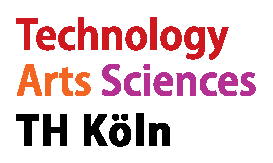
\includegraphics[scale=1.00]{Sources/logo_TH-Koeln_CMYK_22pt}\\
    \begin{center}
      \Large
      Technische Hochschule Köln\\
      Fakultät für Informatik und Ingenieurwissenschaften\\
      \hrule\par\rule{0pt}{2cm} % Horizontale Trennlinie  mit 2 cm Abtand nach unten erzeugen
      \LARGE
      \textsc{B A C H E L O R A R B E I T}\\
      \vspace{1cm} % Vertikaler Abstand von 1cm erzeugen
      \huge
      Der Einfluss von Farbnormalisierung auf die Klassifizierung von Bildern durch künstliche neuronale Netze\\
      \Large
      \vspace{1 cm}
      \large
      Vorgelegt an der TH Köln\\
      Campus Gummersbach\\
      im Studiengang\\
      Medieninformatik\\ 
      \vspace{1.0cm}
      ausgearbeitet von:\\
      \textsc{Torben Krause}\\
      (Matrikelnummer: 11106885)\\
      \vspace{1.5cm}
      \begin{tabular}{ll} % Einfache Tabelle ohne Rahmen, mit 2 Spalten erzeugen
          \textbf{Erster Prüfer:} & Professor Dr. Martin Eisemann \\
          \textbf{Zweiter Prüfer:} & Professor Dr. Matthias Böhmer \\
      \end{tabular}
      \vspace{1.5cm}
      \\Gummersbach, im Juli
    \end{center}    
  \end{titlepage}
  
  \newpage
  \section*{Vorwort}
  \section*{Danksagung}
  \section*{Abstract}
  \newpage
  \listoffigures
  \newpage
  \listoftables
  \newpage
  \tableofcontents
  \newpage
  \section{Einleitung}\label{s.einleitung} 
In keinem Zeitabschnitt waren digitale Technologien so stark im Fokus wie heutzutage. Gerade der Bereich selbstständig lernender Computer wird in der Forschung untersucht und vorangetrieben. Auch bekannt unter dem Namen \textit{Deep Learning} oder künstliche Intelligenz (KI), ist mit diesen Bezeichnungen meist der Bereich der künstlichen neuronalen Netze gemeint. Solche Netze können durch eingeführte Datensätze oder Regeln lernen. Dadurch werden sie in dem trainierten Bereich \textit{intelligent}. Durch genügend Beispiele in den Trainingsdaten können sie Hypothesen aufstellen. Die Faktoren, welche beim Training wichtig sind, stellen zum einen die Menge, wie auch die Qualität der Trainingsdaten dar, zum anderen die Zeit, in welcher das neuronale Netz trainiert wird. Durch steigende Rechenleistung kann das Verfahren beschleunigt werden, da normalerweise viel Zeit für das Training benötigt wird. In der Vergangenheit konnten die Forschungen durch zu langsame Hardware nicht effektiv weiter geführt werden. Mit der Leistung heutiger CPUs und GPUs ist dies ohne Probleme möglich.\\ 
  \subsection{Problemstellung und Ziele}\label{s.probuziel} 
Beim Erstellen eines neuronalen Netzes könnnen durch schlechte Trainigsdaten Schwierigkeiten entstehen. Im Bereich der Objekterkennung können dadurch Probleme, wie fehlerhafte Zuordnungen auftreten. Datensätze bestehen üblicherweise aus mehreren Hunderttausend Bildern und bei Vortrainierten um die Tausend Bilder. Die richtige Ausleuchtung ist ein wichtiger Aspekt bei der Generierung der Trainingsbilder, da schon kleine Veränderungen der Lichtverhältnisse die Farben der Objekte verändern können. Ein und dasselbe Objekt kann dadurch in vielen verschiedenen Farbvariationen auftreten, wie man in Abbildung \ref{img:problem} erkennen kann. Durch weniger licht wirken die Farben dunkler und unterscheiden sich sichtlich. Gerade bei einem Datensatz mit wenig Bildern, kann das zu fehlerhaften Prognosen führen. Häufig kann eine konstante Ausleuchtung nicht gewährleistet werden, weil die Bilder in der freien Umwelt erstellt werden und eine Ausleuchtung zu umständlich wäre. Das bedeutet das dieses Problem hauptsächlich in der Nachbereitung der Bilder angegangen werden kann.
\begin{figure}
	[h]
	\centering
	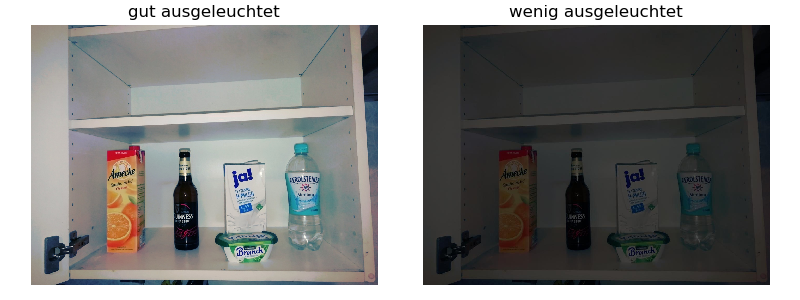
\includegraphics[scale=0.7]{Sources/Vergleich.png}
	\caption{Szene mit unterschiedlicher Ausleuchtung}
	\label{img:problem}
\end{figure}\\
  \subsection{Erläuterung der These}\label{s.these}
Für solche Probleme bietet die Bildverarbeitung einige Lösungsansätze, welche von der Theorie aus, eine konstante Farbgebung und dadurch eine Erhöhung der Genauigkeit bringen könnten. Ob es in der praktischen Ausführung die erwarteten Ergebnisse erzielt, soll getestet werden. Deswegen sollen in dieser Arbeit verschiedene Verfahren der Farbnormalisierung von Bildern auf die Trainings- und Testdatensätze angewendet und auf verschiedene künstliche neuronale Netze trainiert werden. Beim Vergleich der Trainingsergebnisse soll herausgestellt werden, ob das Normalisieren der Daten einen positiven Einfluss auf die Genauigkeit hat und welche Unterschiede die Normalisierung-Verfahren aufweisen.\\
  \subsection{Anforderungen}\label{s.anforderungen}
Bei dem geplanten Vorhaben, welches diese Arbeit thematisiert, ist es wichtig Anforderungen an das neuronale Netz, dem Datensatz und den verwendeten Algorithmen zu formulieren, um sicher zu stellen, das keine vermeidbaren Probleme auftreten. Zunächst werden Trainingsdaten benötigt, mit welchen die neuronalen Netze trainiert werden. Viele wissenschaftliche Arbeiten zeigen, dass eine große Menge an Daten benötigt wird, um ein gut funktionierendes neuronales Netz zu entwickeln. Im Schnitt werden 50.000 Trainingsbilder pro Klasse benötigt. Diese Menge an Daten kann im Anbetracht der verfügbaren Zeit nicht für drei verschiedene Datensätze generiert werden. Da die benötigten Ressourcen nicht zur Verfügung stehen, soll eine Möglichkeit gefunden werden, gute Ergebnisse mit einer geringeren Menge an Trainingsdaten zu realisieren. Um genügend Vergleichswerte untersuchen zu können, sollen mehrere Datensätze mit unterschiedlichen Klassen genutzt werden. Um sicher zu stellen, dass die Datensätze zum Vorhaben geeignet sind, werden diese für die Arbeit erstellt und ausgesucht. Da diese für die Arbeit geeignet sein müssen, ist es wichtig, eine hohe Qualität an Daten zu verwenden.\\\\
Die Trainingsdaten sollen unter folgenden Anforderungen erstellt werden:
\begin{enumerate} 
\item Ein qualitativ hochwertiger Datensatz sollte nicht unordentlich sein, da das Reinigen der Daten lange dauern kann. ??? Anforderungen zu schwammig, was heißt unordentlich, was bedeutet reinigen? ???
\item Der Datensatz sollte nicht zu große Daten enthalten, da sie den Trainingsfortschritt zurückhalten und mehr Ressourcen benötigen. ??? Was sind zu große daten, is damit die auflösung gemeint???
\item Beim Generieren der Trainingsbilder sollte darauf geachtet werden saubere und gut ausgeleuchtete Aufnahmen zu machen. ??? Was bedeutet sauber ?? 
\item Das Ziel des Datensatzes sollte gut Definierte werden.
\end{enumerate}
Um die Auswirkungne der Normalisierungsverfahren vergleichen zu können werden verschiedene Verfahren auf die selben Trainings- und Testdaten angewendet. Durch die Normalisierungsverfahren soll die Farbvarianz verringert werden ???? Anwendung der Normaliesirung auf Trainigsdaten oder Testdaten oder beiden ??? .
  \subsection{Struktur der Arbeit}\label{Struktur}
??? ich würde mit dem Digital Bild beginnen ??? 
Für ein besseres Verständnis der einzelnen Entwicklungsschritte in den späteren Kapiteln werden in Kapitel ??? zuerst die Grundlagen der künstlichen neuronalen Netze beschrieben. Hierbei werden die unterschiedlichen Schichten welche durchlaufen werden aufgeführt und beschrieben. Im Weiteren wird auf die digitale Bildverarbeitung eingegangen. Dabei soll zunächst vermittelt werden wie digitale Bilder entstehen und aus welchen Komponenten diese zusammengesetzt sind. Anschließend werden die verwendeten Farbnormalisierungsverfahren erklärt und beschrieben ??? Vergleichen.\\\\
In der zweiten Hälfte der Arbeit wird es um die Durchführung des praktischen Teils der Arbeit gehen. In diesem wird zunächst die Grundlage aufgeführt, auf welcher das Training durchgeführt wurde. Die verwendeten Farbnormalisierungsverfahren werden zusätzlich in der technischen Umsetzung erläutert. Zum Schluss kommt es zur Durchführung des Trainings der verschiedenen Netze, welche daraufhin verglichen und ausgewertet werden. In einer Diskussion wird nun das Ergebnis der Auswertung anhand der angeführten These evaluiert und ein Fazit der Arbeit getroffen.
  \newpage
  \section{Theoretische Grundlagen}\label{s.grundlagen}
  Das folgende Kapitel soll eine kurze und leicht verständliche Einführung sein, in dem die Theoretischen Grundlagen über den Aufbau von digitalen Bildern der einfluss von Belichtung sowie den verwendeten Bildbearbeitung Methoden gelegt. Anschlißend folgt ein Überblick über die Grundlagen der künstlichen Intelligen. Der letzte Abschnitt wittmet sich den Schwerpunkten der künstlichen neuronalen Netze. Dabei werden hauptsächlich für die Arbeit relevante Grundlagen vermittelt. 
  \subsection{Digitale Bilder}\label{s.digibilder}
  Damit der Ansatz der These, dass die Farbnormalisierung von Trainingsdaten das Trainingsverhalten und die spätere Genauigkeit künstlicher neuronaler Netze verbessern kann, nachvollzogen werden kann, soll in diesem Unterkapitel, auf die Aufnahme digitaler Bilder, mit deren Eigenschaften und Aufbau eingegangen werden. Außerdem sollen die Schwächen herausgearbeitet und mögliche Lösungsansätze erläutert werden. Zunächst folgt eine kurze Einführung.\\\\
  Noch vor einiger Zeit war die Aufnahme und Verarbeitung von Bildern nur einer kleinen Gruppe von Spezialisten, mit kostspieliger Ausrüstung möglich. Spätestens seid der Entwicklung von digitalen Aufnahmegeräten wie Digitalkameras, Scannern und Multimedia-PCs ist die Aufnahme und Verarbeitung von Bildern, nicht mehr einer kleinen Gruppe von Spezialisten vorbehalten, sondern für jeden erschwinglich. Mittlerweile gibt es eine riesige Community von Menschen, bei denen das Arbeiten mit digitalen Bildern schon längst zum Alltag geworden sind. Durch heutige Bildverarbeitungsprogramme wird ein tiefer gehendes Wissen nicht mehr zwingend vorausgesetzt, denn viele komplexen Abläufe werden automatisiert. Das führt zu dem Problem, das Aufbau und zusammenhänge der Bilder häufig nicht verstanden und falsch genutzt werden. Auch im professionellen Bereich wie, Werbung, Medizin, Deep Learning, werden fast ausschließlich digitale Bilder verwendet. Auch hier entstehen oft, durch das fehlende Verständnis der Zusammenhänge, häufig zur Unterschätzung der Probleme und nicht selten zu ineffizienten Lösungen, teuren Fehlern und persönlicher Frustration.\\
  Bildverarbeitung, wird in der heutigen Zeit oft mit Bildbearbeitung assoziiert, also mit der Bearbeitung von Bildern mittels Bearbeitungssoftware. In der Bildverarbeitung geht es anders als in der Bearbeitung, um die Software selber, welche für die Konzeption und Erstellung von digitalen Bildern genutzt wird. In der Programmierung sind Bilder nichts weiter als Zahlen-Matrizen ??wie in Abbildung ... ein bild von einem Graustufen Bild und seiner Matrix (3x3)  könnte hier gut sein??? , welche man nach Belieben lesen und verändern kann, um seine geplanten Ziele zu erreichen. Grundsätzlich bestehen digitale Bilder aus rastern. Diese besitzen mehrere werte, welche auch Pixel genannt werden. In diesen Pixeln werden Bildinformationen wie Farbe und Position festgehalten. Jeder Pixel besteht dabei oft aus drei Kanälen, den R Kanal für Rot, den G Kanal für Grün und den B Kanal für Blau. Diese bilden in bestimmten Kombinationen und Intensitäten ungefähr 16 Millionen verschiedene Farben. Der beschriebene Aufbau wird bei RGB-Bildern verwendet und auch bei Monitoren, Smartphones, etc. Neben dem RGB gibt es noch einige verschiedene Farbräume (CMY, CMYK, HSV, Lab, etc).\\\\
  \textbf{RGB}\label{s.rgb}\\
  Der RGB-Farbraum ist der geläufigste und bekannteste Farbraum dieser besteht wie in () ??? Verweiß fehlt ??? kurz beschrieben aus drei Farbräumen (Rot-Grün-Blau). Dieses beschreibt, welche Art von Licht ausgestrahlt werden muss, um eine gewünschte Farbe zu erreichen. Die Kombination der einzelnen Farbräume ist eine additive Farbmischung. RGB ist eher ein Farbmodell, da es viele Farbräume gibt, welche sich davon Ableiten (sRGB, AdobeRGB, etc.).\\\\
  \textbf{HSV}\label{s.hsv}\\
  Anders als der RGB ist der HSV Farbraum aufgebaut, dennoch gibt es auch hier drei Werte. Das H (Hue) seht für den Farbton, welcher angenommen werden soll, S (Saturation) für die Sättigung der ausgewählten Farbe und V (Value) für den Hell-wert oder auch die Helligkeit der Farbe. Der HSV Farbraum besteht aus diesen Koordinaten. Dieser Farbraum ist gerade in der Kunst beliebt, da die Farbvorstellung besser funktioniert als bei additiven und subtraktiven Farbmischungen.\\\\
  \textbf{CMY/CMYK}\label{s.cmy}\\
  Anders als der RGB-Farbraum benutzt der CMY-Farbraum den subtraktiven anstelle der additiven Farbmischung. Hierbei sind die drei Grundfarben C für Cyan, M für Magenta und Y für Yellow. Bekannt ist diese Farbmischung gerade durch das Malen von Wasserfarben, oder für die Farbpigmente, welche in Druckern genutzt werden. Für den durch die Farbmischung kann der CMY kein richtiges Schwarz erreichen, deswegen wurde der Farbraum CMYK mit einem Parameter erweitert. Das K steht für Schwarz, damit auch schwarz richtig dargestellt werden kann und kein dunkles Grau entsteht.\\\\
  \textbf{Lab}\label{s.lab}\\
  Der Lab-Farbraum ist ein Messraum, in welchem jede wahrnehmbare Farbe enthalten ist. Der Farbraum wurde auf Grundlage der Gegenfarbentheorie konstruiert. Eine wichtige Eigenschaft, ist die Geräteunabhängigkeit. Das bedeutet, die Farben werden unabhängig der Erzeugung und der Wiedergabe definiert. Die umfassende Definition kann in der DIN 6174 nachgelesen werden. Auf Grundlage der Gegenfarbentheorie liegen sich auf der a Achse die Farben Grün und Rot gegenüber. Die b Achse entspricht den Gegenfarben Blau und Gelb. Senkrecht durch die Ebenen befindet sich die L Achse welche von 0 (weiß) bis 100 (Schwarz) geht. Diese gibt die Helligkeit wieder und hat Zwischenschritte für die Graustufen.
    \subsubsection{Aufbau von Digitalbildern}\label{s.aufbdigibilder}
  Üblicherweise wird bei Digitalbildern mit dem RGB-Farbraum gearbeitet. Aus diesem Grund, wird in dieser Arbeit hauptsächlich auf RGB-Bilder eingegangen. Ein Bild ist wie eine Matrix aufgebaut, dabei kann es sowohl quadratisch wie auch rechteckig Abmessungen haben. Jeder Punkt in der Matrix stellt einen Pixel dar und enthält jeweils einen Rot-, grün-, Blauwert welche zusammen eine beliebige Farbe darstellt. Um die Farbverteilung in einem Bild besser erkennen zu können, werden die Farbwerte in sogenannten Farb-Histogrammen zusammengefasst. Histogramme spielen für die Normalisierungsfunktionen eine Rolle, aus diesem Grund wird das Konzept hinter den Histogrammen und die spätere Manipulation, beschrieben. Für die einfachheitshalber werden Graustufenbildern für die Erklärung verwendet. Anwendbar sind diese auch auf die Histogramme der einzelnen RGB-Kanäle.\\\\
  \textbf{Histogramme}\label{s.histogramme}\\
  Histogramme beschreiben eine Häufigkeitsverteilung \cite[42ff.]{burger2009digitale}. Speziell bei Bildern zeigen Histogramme die Häufigkeit der auftretenden Intensität-werte. Am einfachsten lässt sich das mit Graustufenbildern nachvollziehen. Ein Beispiel dafür zeigt die (Abbildung \ref{img:histogramm}) für ein Graustufenbild $I$ mit möglichen Intensität-werten im Bereich $I(n,V)E[0,K-1]$ enthält das Histogramm $H$ genau $K$ Einträge. Die Menge der Einträge bei einem 8 Bit Graustufenbild sind $2^8$ Farbabstufungen ($K=2^8=256$). Der Wert des Histogramms an der Stelle $i$ ist $h(i)$ die Anzahl der Pixel von $I$ mit einem Intensitätswert $i$, für alle ($0<i<K$). Mathematisch ausgedrückt ergibt sich $h(i)=card{(u,v) | I(u,v)=i}$\\
  daraus lässt sich entnehmen, dass $h(0)$ die Anzahl der Pixel mit dem Wert 0, $h(1)$ die Anzahl des Wertes 1 usw., $h(255)$ ist schließlich der letzte Wert und gibt die Menge aller weißen Pixel in dem Bild an $(K-1)$. Eine Histogramm Berechnung stellt somit einen eindimensionalen Vektor $h$ der Länge $K$ da.\\
  \begin{figure}
    [h]
    \centering
    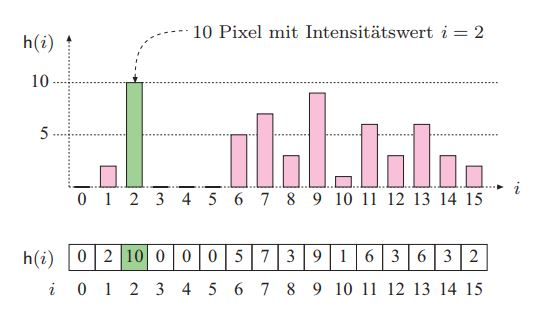
\includegraphics[scale=1.0]{Sources/histogramm.jpg}
    \caption{Histogramm eines Graustufen Bildes mit 16 Helligkeitsabstufungen \cite[42]{burger2009digitale}}
    \label{img:histogramm}
  \end{figure}
  $card$ beinhaltet die Anzahl der Elemente einer Menge (\textit{Kardinalität})\\\\
  Die Abb.\ref{img:histogramm} zeigt ein mögliches Histogramm mit einer Farbabstufung von 16 werten. Ein Histogramm zeigt die wichtigsten Eigenschaften eines Bildes, wie beispielsweise die Dynamik oder den Kontrast eines Bildes. Außerdem lässt sich erkennen, ob bei der Bildaufnahme Probleme aufgetreten sind. Diese lassen sich erkennen indem Ausschläge ganz links oder ganz rechts, des Graphen zu erkennen sind. Ein Ausschlag bei 0 oder 255 bedeutet das dort keine Farbinformationen mehr vorhanden sind, und das teile des Bildes, Über- beziehungsweise unterbelichtet sind.\\\\
  \textbf{Kontrast}\label{s.kontrast}\\
  Der Kontrast bezeichnet den Bereich von Intensitätstufen, welche in einem Bild effektiv genutzt werden, also die Differenz der maximalen und minimalen Pixelwerten \cite[44]{burger2009digitale}. Ein Bild welches einen hohen Kontrast hat, nutzt das gesamte Spektrums des Histogramms (Schwarz bis weiß). Der Kontrast, lässt sich also leicht aus einem Histogramm entnehmen, wie in Abb. (NOCH HINZUFÜGEN) die verschiedenen Histogramme zeigen.\\\\
  \textbf{Dynamik}\label{s.dynamik}\\
  Dynamik bedeutet, wie viel verschiedene Pixelwerten in einem Bild genutzt werden, und die jeweilige Anzahl\cite[44]{burger2009digitale}. Im besten Fall entspricht die Dynamik der insgesamt genutzten Anzahl an Pixelwerten. Also $K-1$ genutzter Farbabstufungen, damit der Wertebereich voll ausgeschöpft wird.\\\\
  Anders als der Kontrast, welcher immer erhöht werden kann, solange der maximale Wertebereich nicht erreicht worden ist, kann die Dynamik eines Bildes nicht so leicht verbessert werden. Aus diesem Grund ist eine hohe Dynamik von Vorteil, denn dadurch wird die Gefahr von Qualitätsverlust bei Verarbeitungsschritten verringert. Trotz der Tatsache, das viele Ausgabegeräte mit Farbtiefen von 8 Bit arbeiten, nehmen heutige Kameras bis zu 12-14 Bit pro Kanal auf, um einen möglichen Qualitätsverlust vorzubeugen.
    \subsubsection{Einfluss von Belichtungen}\label{s.belichtung}
  In dem Kapitel\ref{s.aufbdigibilder} wurde Beschrieben wie die Farben in Bildern gespeichert werden und welche unterschiedlichen Arten von Farbräumen es gibt \cite[41ff.]{burger2009digitale}. Bei der Aufnahme von Bildern ist gerade die Belichtung entscheiden. Eine hohe Belichtung sorgt dafür, dass Farben heller wirken, wobei wenig licht dafür sorgt das Farben dunkler erscheinen. Diese Tatsache kann beim Deep Learning zu Problemen führen, da ein und dasselbe Objekt unterschiedliche Farben annehmen kann und je nach Belichtungsintensität variiert. Ein künstliches neuronales Netz kann Objekte welche es normalerweise trainiert hat nicht immer erkennen, wenn die Farbe zu stark von der eigentlichen Farbe abweicht. Um Belichtungen auf Bildern auszugleichen und zu normalisieren, gibt es einige verfahren, welche diesem Problem entgegenwirken. Die Ausgewählten verfahren werden aufgeführt und beschrieben. Diese stellen nicht die Originalfarbe des Objektes wieder her, sondern sorgen für eine konstante Farbvariation, welche sich nicht stark verändert.
    \subsubsection{Arten der Farbnormalisierung}\label{s.farbnormalisierungen}
  Die Farbnormalisierung ist ein Thema der Bildverarbeitung und wird hauptsächlich mit künstlicher Farbsicht befasst. Die Verteilung und Darstellung von Farben auf Bildern hängt hauptsächlich von Beleuchtungsbedingungen und der Kamera ab. Das bedeutet das sich die Farben bei der Aufnahme, je nach Beleuchtung verändern. Das ist gerade im Bereich von \textit{Maschine Learning} problematisch, da diese Farbveränderungen zu Fehlern im Lernprozess und der späteren Genauigkeit führen. Farbnormalisierung-Algorithmen, sollen dafür sorgen, dass die Farbabweichungen durch Lichteinfluss geringere Auswirkungen habe und zu besseren Ergebnissen führen. Im folgenden werden die ausgewählten Algorithmen erläutert, welche im Rahmen dieser Arbeit getestet werden.\\\\
  \textbf{Gray-World-Algorithmus}\label{s.gw}\\
  Bei der Gray-World Normalisierung geht es nicht, wie der Name vermuten lässt um die Umwandlung in ein Graustufenbild, eher werden die verschieden Farbräume abgedunkelt und eingegrenzt. Es wird davon ausgegangen, dass das Farbspektrum durch drei konstante Faktoren modelliert werden kann. Dafür skalieren die Konstanten $\alpha$, $\beta$ und $\gamma$ an die Kanäle R, G und B. Dadurch kann eine Konstanzlösung erzielt werden, welcher bei unterschiedlichen Belichtungen unveränderlich ist, indem jeder Farbkanal durch seinen Durchschnittswert geteilt wird, wie in folgender Formel beschrieben:\\
  \begin{eqnarray} (\alpha R, \beta G, \gamma B) \rightarrow\left(\frac{\alpha R} {\frac{\alpha}{n} \sum_{i} R}, \frac{\beta G} {\frac{\beta}{n} \sum_{i} G}, \frac{\gamma B} {\frac{\gamma}{n} \sum_{i} B} \right) \end{eqnarray}\\
  Wie schon erwähnt, ist diese Art der Farbnormalisierung für verschiedene Farbvariationen unveränderlich. Ein größeres Problem dieses Normalisierung-verfahren besteht darin, das nicht alle Variationen der Beleuchtungsintensität berücksichtigt und auch nicht einfach für dynamische Szenen verwendet werden kann. Um solche Probleme zu lösen, gibt es mehrere Variationen dieses Algorithmus.\\\\
  \textbf{Histogramm Ausgleichung}\label{s.ha}\\
  Die Histogramm Ausgleichung ist eine Nichtlineare Transformation, welche auf Grundlage der Histogramme wie in Kapitel \ref{s.histogramme} beschrieben arbeitet. Der Pixelrang wird dabei nicht verändert und kann bei jeder monoton steigenden Farbformation-Funktion verwendet werden. Diese Normalisierung-Funktion gilt stärker als der Gray-World-Algorithmus. Durch die Histogramm Ausgleichung entsteht ein dominanter blauer Kanal, wodurch das Bild oft unnatürlich erscheint.\\\\
  \begin{table}
  [h]
  \caption{Tabellarisches Histogramm des Zielbildes}
  \centering
  \begin{tabular}{|l|c|c|c|c|c|c|c|c|}
  \hline
  Graustufen & 0 & 1 & 2 & 3 & 4 & 5 & 6 & 7\\
  \hline
  Anzahl der Pixel & 8 & 10 & 10 & 2 & 12 & 16 & 4 & 2\\
  \hline
  \end{tabular}
  \end{table}
  \begin{table}
  [h]
  \centering
  \begin{tabular}{|c|c|c|c|c|c|c|c|}
  \hline
  0&1&5&1&7&2&0&3\\
  \hline
  0&0&5&5&5&2&4&5\\
  \hline
  4&5&1&4&1&5&1&4\\
  \hline
  5&1&2&4&5&2&6&3\\
  \hline
  5&2&6&4&0&4&0&5\\
  \hline
  4&0&2&4&7&4&6&2\\
  \hline
  5&1&6&1&0&1&1&5\\
  \hline
  4&3&2&4&2&5&2&5\\
  \hline
  \end{tabular}
  \end{table}\\
  Aus der Pixelverteilung wird nun ein Ausgleich berechnet welche den kumulativen Pixelwert durch die Anzahl aller Pixel teilt und durch die höchste Graustufe teilt. Das Ergebnis wird gerundet und der passenden Graustufe zugeordnet. Die Vorgehensweise mit Farbbildern funktioniert gleich, nur das die R, G und B Kanäle verwendet werden.
  \begin{table}
  [h]
  \caption{Mathematische Umsetzung der Histogrammausgleichung}
  \centering
  \begin{tabular}{|l|c|c|c|c|}
  \hline
  $r_{k}$ & $P_{k}$ & Kumulative Werte & $Kumulative/Gesamt*(L-1)$ & Gerundete nahe Grauwerte\\
  \hline
  0 & 8 & 8 & $8/64*7=0.875$ & 1\\
  \hline
  1 & 10 & 18 & $18/64*7=1.968$ & 2\\
  \hline
  2 & 10 & 28 & $28/64*7=3.0625$ & 3\\
  \hline
  3 & 2 & 30 & $30/64*7=3.2812$ & 3\\
  \hline
  4 & 12 & 42 & $42/64*7=4.5937$ & 5\\
  \hline
  5 & 16 & 58 & $58/64*7=6.3437$ & 6\\
  \hline
  6 & 4 & 62 & $62/64*7=6.78125$ & 7\\
  \hline
  7 & 2 & 64 & $64/64*7=7$ & 7\\
  \hline
  \end{tabular}
  \end{table}\\
  \textbf{Histogramm Spezifikation}\label{s.hs}\\
  Ähnlich wie die Histogramm Ausgleichung arbeitet die Histogramm Spezifikation. Die Histogramme der roten, grünen und blauen Kanäle werden so umgewandelt, dass sie den Formen von drei spezifischen Histogrammen entsprechen, anstatt sie einfach auszugleichen. Mithilfe dieses Vorgehens wird darauf abgezielt, Bilder zu erhalten welche ein Histogramm einer bestimmten Form haben. Zunächst muss das Bild so konvertiert werden, dass das Histogramm eine bestimmte Form hat.
  Für diese Methode werden üblicher weise zwei ähnliche Bilder verwendet, einmal das Hauptbild und das Referenzbild. Das Referenzbild hat die gewünschte Form des Histogramms, hingegen das Hauptbild nicht optimiert ist. Zunächst wird mit beiden Bildern eine Histogramm Ausgleichung durchgeführt. Im Weiteren wird das Referenz-Histogramm mit dem des Hauptbildes kombiniert und angepasst.\\\\
  \begin{table}
  [h]
  \caption{Tabellarisches Histogramm des Quell-Bildes (B1)}
  \centering
  \begin{tabular}{|l|c|c|c|c|c|c|c|c|}
  \hline
  Graustufen & 0 & 1 & 2 & 3 & 4 & 5 & 6 & 7\\
  \hline
  Anzahl der Pixel & 8 & 10 & 10 & 2 & 12 & 16 & 4 & 2\\
  \hline
  \end{tabular}
  \end{table}\\
  \begin{table}
  [h]
  \caption{Tabellarisches Histogramm des Referenz-Bildes (B2)}
  \centering
  \begin{tabular}{|l|c|c|c|c|c|c|c|c|}
  \hline
  Graustufen & 0 & 1 & 2 & 3 & 4 & 5 & 6 & 7\\
  \hline
  Anzahl der Pixel & 0 & 0 & 0 & 0 & 20 & 20 & 16 & 8\\
  \hline
  \end{tabular}
  \end{table}\\
  Um die Funktionsweise verständlicher darzustellen, wird kurz auf das Vorgehen und die mathematische Herleitung eingegangen. Dafür gibt es in den Tabellen?und? zwei Histogramme mit 8 Grauabstufungen. In diesen Tabellen wird aufgeführt, wie oft der jeweilige Grauwert in dem Bild vorkommt. Nun werden die Histogramme wie in Absch\ref{s.histogramme} beschrieben, ausgeglichen. Von 0 bis $L-1$ werden die Summen der Pixel berechnet, durch die Anzahl der im Bild enthaltenden Pixel geteilt und mit der höchsten Graustufe $(L-1)$ multipliziert. Das Ergebnis des Ausgleiches wird in Tabelle? Aufgeführt. Nun werden die Grauwertverteilungen von B1 und die Verteilung von B2 angepasst dafür wird der nächste Wert aufgerundet von B1 übernommen.\\\\
  In einem Beispiel:
  
  1 (B1) am nächsten an 2 (B2) liegt bei Graustufe 4
  
  2 (B1) am nächsten an 2 (B2) liegt bei Graustufe 4
  
  3 (B1) am nächsten an 4 (B2) liegt bei Graustufe 5
  
  3 (B1) am nächsten an 4 (B2) liegt bei Graustufe 5
  
  ......\\
  \begin{table}
  [h]
  \caption{Von zwei Ausgeglichenen Histogrammen zu einem Spezifizierten Histogramm}
  \centering
  \begin{tabular}{|c|c|c|c|}
  \hline
  Graustufe & Ausgleichung B1 & Ausgleichung B2 & Spezifiziertes Histogramm\\
  \hline
  0 & 1 & 0 & 4\\
  \hline
  1 & 2 & 0 & 4\\
  \hline
  2 & 3 & 0 & 5\\
  \hline
  3 & 3 & 0 & 5\\
  \hline
  4 & 5 & 2 & 6\\
  \hline
  5 & 6 & 4 & 6\\
  \hline
  6 & 7 & 6 & 7\\
  \hline
  7 & 7 & 7 & 7\\
  \hline
  \end{tabular}
  \end{table}\\
  Aus der neuen Stufen Verteilung entsteht ein neues Histogramm welches weniger Farbstufen enthält. Dadurch verschiebt sich das Histogramm Richtung weiß und das Bild wird erhellt.
  \begin{table}
  [h]
  \caption{Tabellarisches Histogramm des Quell-Bildes (B1) auf Basis des Referenz-Bildes (B2)}
  \centering
  \begin{tabular}{|l|c|c|c|c|c|c|c|c|}
  \hline
  Graustufen & 0 & 1 & 2 & 3 & 4 & 5 & 6 & 7\\
  \hline
  Anzahl der Pixel & 0 & 0 & 0 & 0 & 18 & 12 & 28 & 6\\
  \hline
  \end{tabular}
  \end{table}\\

  \subsection{Künstliche Intelligenz}\label{s.ki}
Künstliche Intelligenz wird heute immer mehr von Firmen und Wissenschaft genutzt. In den letzten Jahren hat die nutzung von künstlichen Inteligenzen enorm zugenommen und Firmen nutzen diese Technologie beispielsweise für die analyse und vohersage von Kundenverhalten, für die Klassifikation von Bildern oder zur Spracherkennung in heutigen Smartphones. Mit künstlicher Intelligenz beschreibt man solche Computer, welche gewisse Aufgaben erledigen, ohne ausdrücklich dafür programmiert worden zu sein. Dabei werden Informationen anhand von Vergleichsdaten dem System zugeführt, wodurch er sich Eigenschaften und Strukturen merkt und durch diese Rückschlüsse und Prognosen ziehen kann. Eine gute Beschreibung geben dabei die Autoren Rich und Knight, in dem sie schreiben:\\\\
 \textit{Das Studium des Problems, Computer dazu zu bringen, Dinge zu tun, bei denen ihnen momentan der Mensch noch überlegen ist.} - (Rich und Knight 1991)\\\\
Ein gutes Beispiel in welchem man das Potenzial von künstlicher Intelligenz sehen kann, ist die Spiele KI  \textit{AlphaGo}. Diese KI wurde von Google entwickelt und ist auf das Spielen des Brettspiels Go trainiert. So konnte \textit{AlphaGo} in einem Match 2016, den damaligen Weltmeister in Go \textit{Lee Sedol} schlagen \cite{Alpha2016GO}. In vier von fünf spielen gewann der Computer. Solche Ergebnisse konnten bis zu diesem Zeitpunkt mit anderen Methoden nicht erzielt werden, da es für damalige Algorithmen zu viele mögliche Spielzüge gab. Durch Deep Learning konnte der Computer ohne feste Algorithmen, besser als der Weltmeister seine Spielzüge Planen. Anhand der Definition von Rich kann man feststellen, dass  \textit{AlphaGo}  im Bereich des Spieles Go als intelligent zählt, da sie dem besten Go-Spieler der Welt deutlich überlegen war.
  \subsection{Neuronale Netze}\label{s.neuronalenetze}
Um das Konzept hinter den künstlichen neuronalen Netzen besser verstehen zu können, betrachten wir zunächst wie der Lernprozess eines Menschen abläuft. Menschliches Lernen ist das Verändern der eigenen Verhaltensstrukturen und die Folgen individueller Erfahrungen \cite{hoffmann2016lern}. Der Lernprozess, kann sowohl bewusst, so wie auch unbewusst unser Verhalten verändern. Menschen adaptieren also die eigenen als auch fremde Erfahrungen zu ihren Gewohnheiten. Diese Prozesse Finden im Gehirn statt, welches aus vielen Nervenzellen besteht. Diese Nervenzellen werden Neuronen genannt und sind untereinander verknüpft, weshalb auch von einem neuronalen Netz gesprochen wird. Maschinelles Lernen nimmt sich also die Funktionsweise des menschlichen Gehirns zum Vorbild \cite[]{ertel2013grundkurs}.\\\\
\textbf{Menschliches lernen}\\
Wie bereits erwähnt, sind der Aufbau sowie die Funktionsweise von künstlichen neuronalen Netzen vom menschlichen Gehirns abgeleitet. Das Gehirn besteht aus ungefähr $10^{11}$ Nervenzellen, welche untereinander verknüpft sind \cite[265ff.]{ertel2013grundkurs}. Für den Lernprozess sind demnach viele Neuronen nötig. In der Abbildung \ref{img:neuron} kann man den wesentlichen Aufbau eines Neurons sehen.
\begin{figure}
	[h]
	\centering
	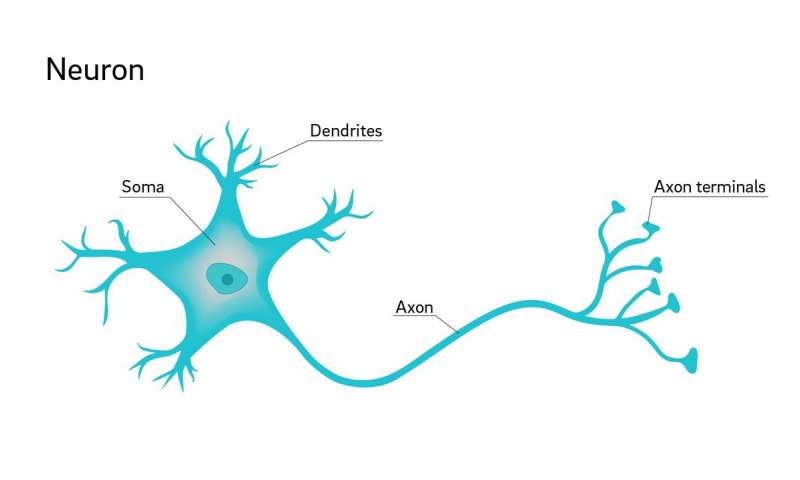
\includegraphics[scale=0.7]{Sources/neuron.jpg}
	\caption{Aufbau eines Neurons \cite{neuron2018UoC}}
	\label{img:neuron}
\end{figure}\\
In diesem vereinfachten Modell eines Neurons lassen sich die wesentlichen Komponenten erkennen. Das Neuron selber besteht aus einem Zellkörper (Soma), einem Axon, den Dendriten auf der linken Seite und den Synapsen(Axon Terminals) auf der rechten Seite. Eine Dendrite stellt mit der Synapse eine Verbindung zu anderen Neuronen her. Diese senden elektrische Impulse an die Soma weiter, welche verarbeitet werden. Wenn die Spannung einen gewissen Schwellwert übersteigt, sendet die Soma einen elektrischen Impuls über das Axon. Jede Synapse sendet das Signal an die Dendriten des nächsten Neurons weiter. Die Stärke des Impulses und der Schwellwert, ist bei jedem Neuron unterschiedlich und verändern sich ständig. Der Schwellwert des Neurons ist niedriger, desto öfter es aktiv ist und steigt wenn es selten aktiv ist \cite{schmidt2013physiologie}. Die aufgeführte Funktionsweise beschreibt nur oberflächlich das Verhalten eines neuronalen Netzes und soll hauptsächlich dem weiteren Verständniss dienen.\\\\
\textbf{Perzeptron}\\
Die Grundlage für den mathematischen Ablauf künstlicher neuronaler Netze wurde von McCulloch und Pitts in ihrem Buch \textit{A logical calculus oft he ideas immanent in nervous activity} erklärt. Auf diesen Grundlagen simulierte 1953 der Psychologe und Informatiker Frank Rosenblatt das erste künstliche Neuron, welches auch als Perzeptron bekannt wurde. In der Abbildung\ref{img:Perzeptron} wird der Aufbau eines solchen Perzeptrons dargestellt.\\
\begin{figure}
	[h]
	\centering
	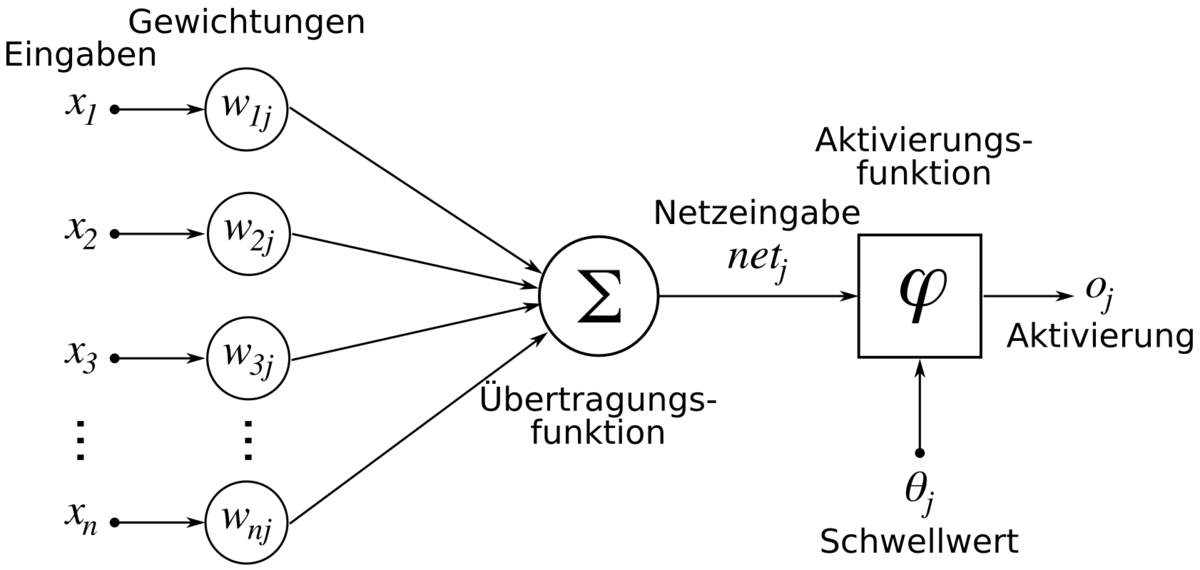
\includegraphics[scale=0.3]{Sources/perzeptron2.png}
	\caption{Schematische Modellierung eines Perzeptrons nach Rosenblatt \cite{perzeptron2019}}
	\label{img:Perzeptron}
\end{figure}\\
Als Eingabewert bekommt das Perzeptron ein Gewicht $w$, welches mit den Eingangswert $x$ multipliziert wird. Das Ergebnis dieser beiden Werte, kann als lineare Funktion beschrieben werden.\\
\begin{eqnarray} f(x) & = & w*x \end{eqnarray}\\
Das Ergebnis der beiden Werte wird an eine Aktivierungsfunktion ??? g??? übergeben. Die Aktivierungsfunktion oder auch Schwellwert genannt, gibt ein Signal weiter, sobald dieser Wert überschritten wird.\\
\begin{eqnarray} g( \sum_{i=0}^n x_{i} *w_{i}) \end{eqnarray}\\
Als Aktivierungsfunktion können sowohl lineare als auch nicht linearen Funktionen verwendet werden. Zusätzlich wird dem Ergebnis der Funktion der \textit{Bias} ??? b ??? addiert.\\
\begin{eqnarray} g(( \sum_{i=0}^n x_{i} *w_{i}) +b \end{eqnarray}\\
Der \textit{Bias} ist eine Art zusätzliches Neuron, für das Verringern von Konvergenz-Problemen, welche bei der Approximation der Funktion auftreten können. Der Bias hat immer einen Eingabewert von 1 und ein Gewicht ??? $w_{jb}$ ??? , welches unabhängig der Eingabewerte ist.\\
\begin{eqnarray} Bias = 1*w_{jb} \end{eqnarray}\\\\
Maschinelles Lernen möchte unter anderem Maschinen in die Lage versetzten Objekte, Strukturen oder auch Abläufe anhand von vorher beigebrachten Beispielen eigenständig zu erkennen. Eine Methode um dieses Ziel erreichen zu können sind die künstlichen neuronalen Netze. Diese werden mit Datensätzen des jeweiligen Schwerpunktes trainiert. Es gibt vier grundlegende Methoden ein solches Netz zu trainieren.\\\\
\textbf{Überwachtes lernen}\\
Das überwachte Lernen funktioniert hauptsächlich mit Datensätzen, welche Eingabedaten sowie Ausgabedaten enthalten. Das künstliche neuronale Netz versucht bei Eingabe der Daten, eine Funktion aufzustellen, welche eine Hypothese darstellt. Diese beschreibt um, was es sich bei dem Datensatz handelt. Die Genauigkeit dieser Hypothese kann durch den Vergleich der enthaltenden Ausgabedaten ermittelt werden. Wenn die Möglichkeiten der Ausgaben endlich sind, handelt es sich um eine Klassifizierung (Bsp.: Milch, Orangensaft, Wasser, etc.). Sollten nur zwei Ausgabewerte möglich sein, ist es eine boolsche bzw. binäre Klassifizierung. Eine Zahl als Ausgabe wird als Regression bezeichnet.\\\\
\textbf{Nicht überwachtes lernen}\\
Die zweite Methode wie ein künstliches neuronales Netz trainiert werden kann, ist eine gegenteilige Herangehensweise. Hier werden lediglich die Eingabedaten übergeben. Das neuronale Netz versucht selbstständig auftretende Muster, in den Daten zu erkennen. Als Beispiel könnte man die sinnvolle Zuordnung von Bildern anhand ähnlicher Muster nehmen. Ähnliche Datensätze werden in Kategorien aufgeteilt, jedoch nicht benannt.\\\\
\textbf{Halb überwachtes Lernen}\\
Oft werden die beiden Methoden des überwachten und unüberwachten Lernen kombiniert, so hat man meist einen kleinen Datensatz mit Ein- und Ausgabedaten, welche aber nicht explizit wahr sein müssen und einen Teil nur mit Eingabeinformationen. Diese Methode wird häufig bei Umfragen verwendet, wo nicht klar ist, ob der Proband wahrheitsgemäß antwortet. Dabei kann ein systematischer Fehler entstehen. Daraus ergibt sich eine Mischung aus überwachten lernen mit systematischen Fehler und unüberwachten lernen, bei welchem das Netz nach häufig auftretenden Mustern sucht.\\\\
\textbf{Verstärktes lernen}\\ 
Das verstärkte Lernen arbeitet auf einem Prinzip, mit welchem richtige Entscheidungen belohnt und falsche bestraft werden. Ein bekanntes Beispiel ist ein Netz, welches virtuell eine Rennstrecke ohne Fehler (nicht von der Strecke abkommen) beenden muss. Bei jedem Fehler muss von vorne begonnen werden, bis die Strecke beendet wird. Ein besonders bekanntes Beispiel ist die GO-KI \textit{AlphaGo} \cite{Alpha2016GO}, welche nur durch die Informationen der Spielregeln trainiert wurde. Die KI wurde in diesem Spiel so gut, das sie den Weltmeister \textit{Lee Sedol} 2016 in vier von fünf Partien GO besiegte.\\\\
\textbf{Künstliche neuronale Netze}\\
Nachdem etwas auf die Grundlagen die verschiedenen Lernverfahren eingegangen wurde, soll in diesem Abschnitt der Aufbau künstlicher neuronaler Netzes und die Logik fokussiert werden. Der mathematische Ablauf der Schichten wird in einem späteren Unterkapitel behandelt.\\
\begin{figure}
	[h]
	\centering
	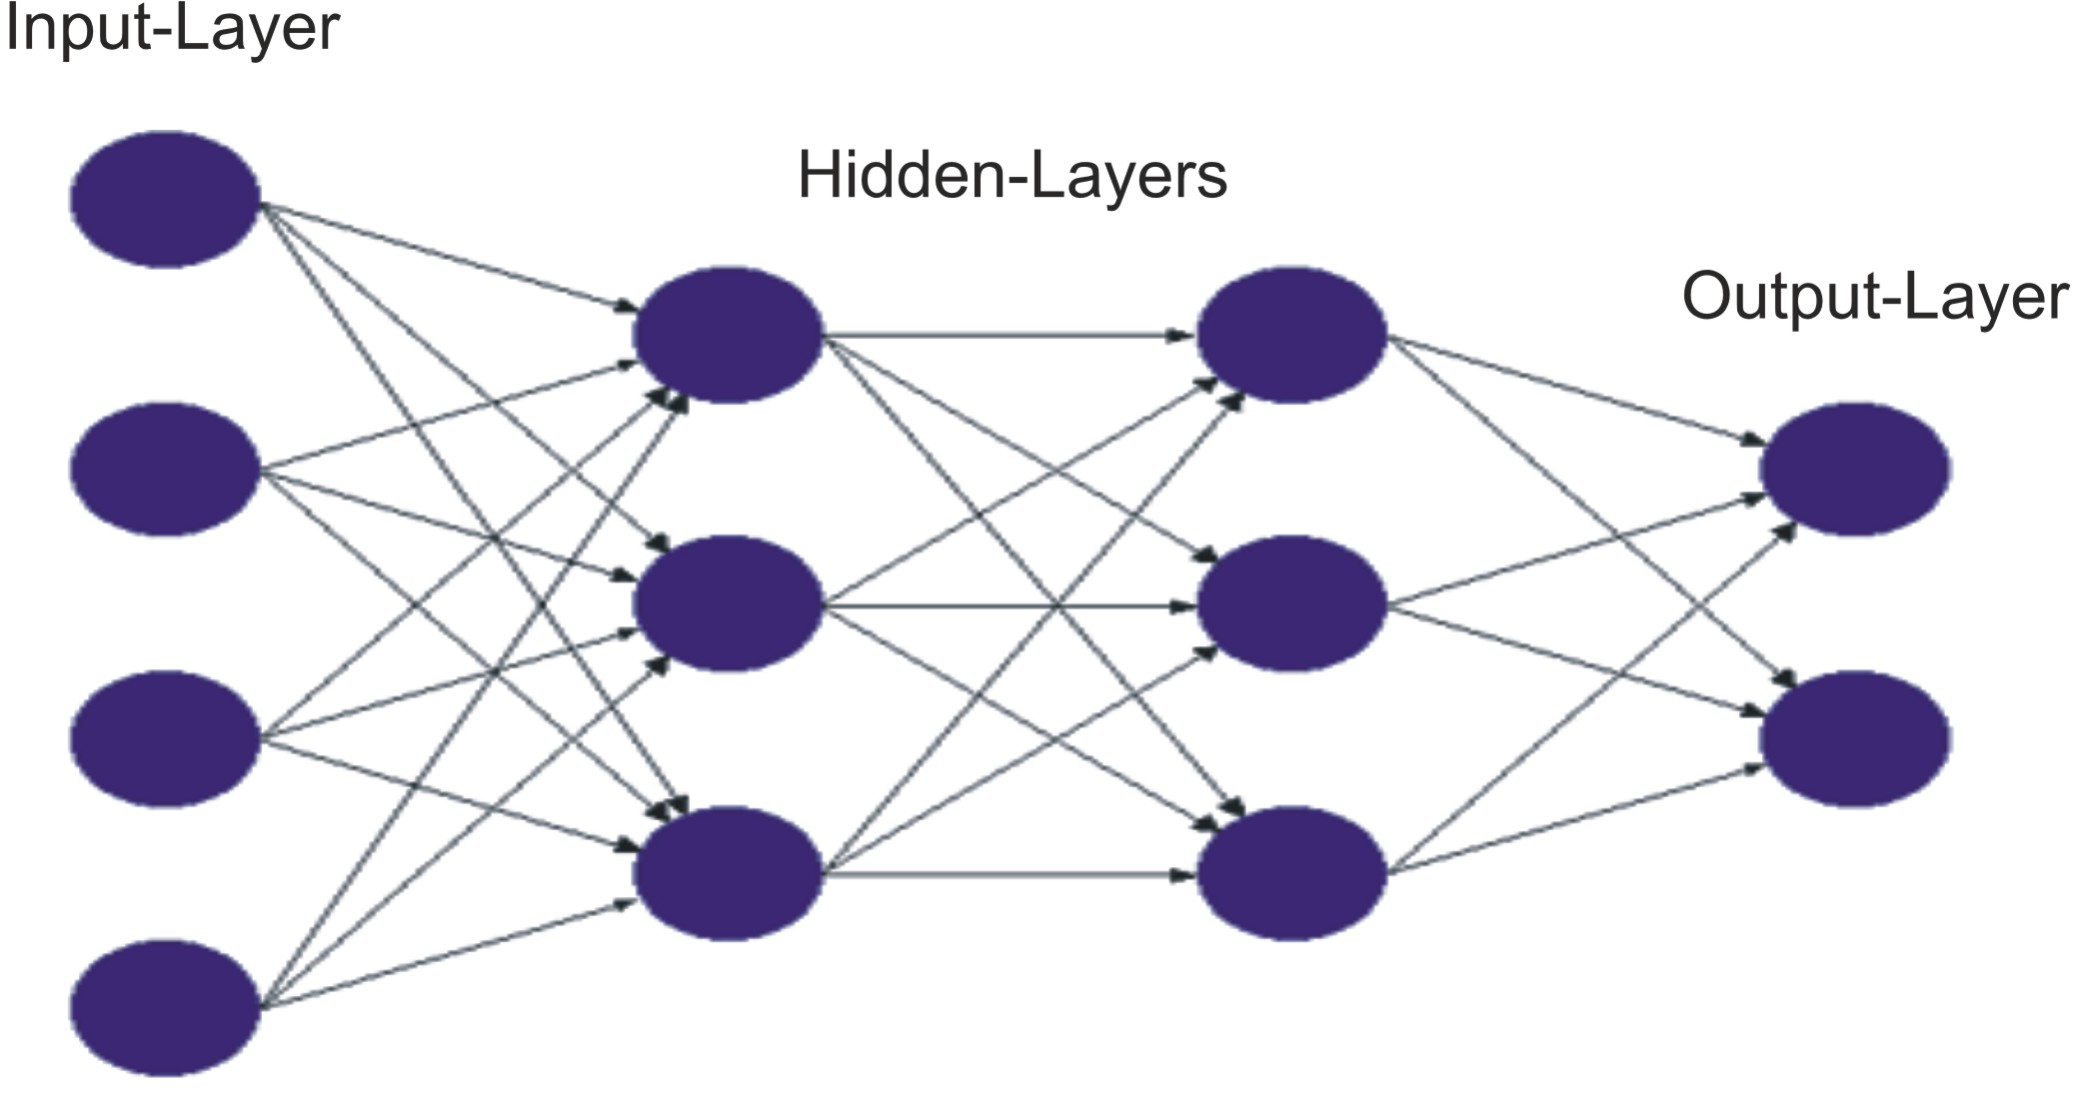
\includegraphics[scale=0.5]{Sources/nnet.png}
	\caption{Aufbau eines künstlichen neuronalen Netzes \cite{bistra2018pic}}
	\label{img:neuronales_netz}
\end{figure}\\
Der Aufbau von klassischen künstlichen neuronalen Netzen kann grundsätzlich in drei Bereiche unterteilt werden. Die erste Schicht stellt der \textit{Input Layer} da. Dieser besteht wie alle folgenden Schichten aus mehreren Neuronen. In diese Schicht werden die Trainingsdaten eingegeben. Jeder wert eines Datensatzes wird mit einem Neuron verbunden. Die Neuronen besitzen eine Gewichtung und einen Schwellwert. Wenn der Schwellwert durch den Eingabewert erreicht wird, sendet das Neuron das Ergebnis seiner Berechnungen an das Neuron der nächsten Schicht weiter. Die folgenden Schichten werden \textit{Hidden Layer} genannt. Die Anzahl der \textit{Hidden Layer} ist variabel und kann so viele Schichten enthalten wie benötigt. Diese Schichten werden auf mehrere verschiedene Merkmale der Eingabedaten trainiert. Dabei werden in frühen Schichten zunächst grobe Strukturen erkannt, welche nach jeder Schicht immer feiner werden. Die letzte Schicht des \textit{Hidden Layer} übergibt seine Informationen an den \textit{Output Layer}. Dieser stellt durch die erhaltenen Daten eine Hypothese auf, in welcher er beschreibt, wie er den Datensatz zuordnet. Dabei gibt das Netz an, zu welcher Wahrscheinlichkeit die Hypothese richtig sein sollte.\\\\
\textbf{Faltende neuronale Netze}\label{s.cnn}\\
\textit{Convolutional neural Networks} oder auch faltende neuronale Netze (Abb. \ref{img:cnn}) sind anders als das KNN, an das Konzept des menschlichen Sehens angelehnt \cite{sermanet2012convolutional} und für das Verarbeiten von matrixartigen Datensätzen konzipiert. Dazu zählen beispielsweise Bildaufnahmen \cite{goodfellow2016deep}. Die erste Schicht besteht aus den \textit{Convolutional Layer}. Bei dieser Schicht wird über die Pixel des Eingabebildes eine Schablone gelegt und vertikal wie auch horizontal verschoben. Diese Schablone hat eine ungerade quadratische Abmessung ($3x3$, $5x5$, $7x7$) und eigene Gewichtungen. Diese Schablone bildet ein Skalarprodukt der unterliegenden Pixel und der Gewichtung. Dabei werden die Strukturen hervorgehoben. Diese Schicht kommt mehrmals in einem Netz vor.\\  
\begin{figure}
	[h]
	\centering
	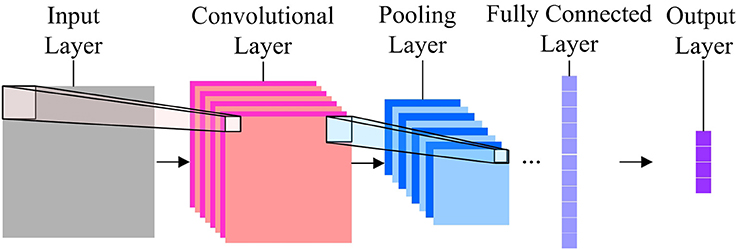
\includegraphics[scale=0.5]{Sources/cnnet.jpg}
	\caption{Aufbau eines Convolutional neural Network \cite{info7040061}}
	\label{img:cnn}
\end{figure}\\
Auf den \textit{Convolutional Layer} folgt immer der \textit{Pooling Layer}. Dieser ist für die Komprimierung des Eingabebildes zuständig, damit im späteren Verlauf Rechenleistung gespart werden kann. Auch diese Schicht besteht aus einer Schablone welches über die Pixel des Bildes gelegt werden. Hierbei werden die Farbwerte der unterliegenden Pixel verarbeitet. Diese werden zu einem wert zusammengefasst und übergeben. Nachdem alle \textit{Convolutional} und \textit{Pooling Layer} durchlaufen wurden, werden die Daten an die letzte Schicht (\textit{Fully Connected Layer}) übergeben. Der \textit{Fully Connected Layer} besteht wie beim KNN beschrieben, aus mehreren Perzeptronen-Schichten und gibt die Informationen an den \textit{Output Layer} weiter, welcher schlussendlich eine Hypothese mit zugehöriger Wahrscheinlichkeit ausgibt.\\\\
\textbf{Loss Funktion}\\
Bei jedem Trainingsschritt versucht das neuronale Netz, eine Hypothese aufzustellen. Damit das Netz Fortschritte im Lernen macht, ist das sogenannte, Backpropagation welches im nächsten Abschnitt genauer beschrieben wird zuständig, welche auf der Basis des Loss Graphen arbeitet. Die Loss Funktion berechnet den Fehler, welcher das Netz in seinem aktuellen Zustand in der Berechnung begeht, also die Differenz zwischen dem Ist- und Sollwert der Ausgabe. Beispiel einer solchen Funktion ist die euklidische Loss-Funktion
\begin{eqnarray} E_{Euclid}&=&\frac{1}{2N} \sum_{n=1}^N || \hat{f_{n}}-f_{n} || \binom{2}{2} \end{eqnarray}
dabei stellt\\

	$\hat{f}_{n}[-\infty,+\infty]$ den berechneten Ist-Wert und
	
	$f_{n}$ den Sollwert dar\\\\
Das Ergebnis der euklidischen Funktion ist das Maß für den Grad der Abweichung von ist und Sollwert.\\\\
\textbf{Rückpropagierung}\\
Die Rückpropagierung oder auch \textit{Backpropagation} \cite{ertel2013grundkurs} ist unter anderem Teil des überwachten Lernens, und beinhaltet das Lernen aus Fehlern. Dadurch das bei einer Klassifizierung Datensätze mit einem Zielwert verwendet werden. Kann das Netz bei einer Zuweisung überprüfen, ob das Ergebnis zu dem Zielwert passt. Dabei wird aus der Ausgabe und dem Zielwert ein Fehler (Loss) berechnet. Sollte das Ergebnis zu weit vom Zielwert abweichen, wird überprüft, welches Perzeptron den größten Einfluss auf die Fehlzuweisung verursacht hat. Dieses Perzeptron wird in seiner Gewichtung angepasst, um den Fehlerwert zu verringern \cite{goodfellow2016deep}. 
??? Mathematische herleitung wie der das Perzeptron bestimmt wird ??? 
  \subsubsection{Funktionsweise künstlicher und Faltender neuronaler Netze}\label{s.funktwknnundcnn}
Die zuvor aufgeführten Netzarten haben einen unterschiedlichen Aufbau und bestimmte Einsatzgebiete. Das Convolutional neural Network ist beispielsweise auf das Verarbeiten von Bilddaten optimiert und Künstliche neuronale Netze eher für serielle Daten. In der Struktur sind die Netzarten ähnlich aufgebaut. Das CNN hat neben den üblichen Neuronenschichten zwei zusätzliche Schichten, welche beim KNN nicht vorhanden sind. In den folgenden Abschnitten soll die Funktionsweise dieser zusätzlichen schichten beschrieben werden.\\\\
\textbf{Faltungsschicht}\\
Es existieren eine menge von Filtern $n$ welche eine Höhe von $f_{h}$ und einer Breite von $f_{w}$ haben. Dieser Filter wird über das Eingabebild mit der Höhe $e_{h}$ und der breite $e_{w}$ gelegt und in ein Pixel schritten bewegt. Die Ergebnisse stellen eine Liste von Merkmalen da welche auf der Höhe $m_{h}$ und der Breite $m_{w}$ liegen. Formell ausgedrückt:\\
\begin{eqnarray} 
m_{h}&=&(e_{h} - f_{h})+1\\
m_{w}&=&(e_{w} - f_{w})+1
\end{eqnarray}\\
Um die Verringerung von Informationen nach der Faltung zu verhindern, werden an den Rändern der Bilder Polsterungen, auch \textit{padding} genannt, angehangen \cite[343]{goodfellow2016deep}. Diese Polsterungen bestehen aus Pixeln mit einem Wert von \textit{0}. Die Anzahl der zusätzlichen Pixel ergibt sich aus der Höhe und Breite des Eingabebildes, um wie viele Pixel das Bild vergrößert wird. Formell ausgedrückt:\\
\begin{eqnarray}
p_{h}&=&f_{h} - 1\\
p_{w}&=&f_{w} - 1
\end{eqnarray}
Die Faltungsschicht hat eigene Gewichte, welche beim Vorgang mit denen des Bildes zusammengerechnet wird \cite[331ff.]{goodfellow2016deep}. Für die gleiche Schicht wird derselbe Filter verwendet. Die Weise der Berechnung wird in der Abbildung \ref{img:faltungsschicht}  beschrieben.\\
\begin{figure}
	[h]
	\centering
	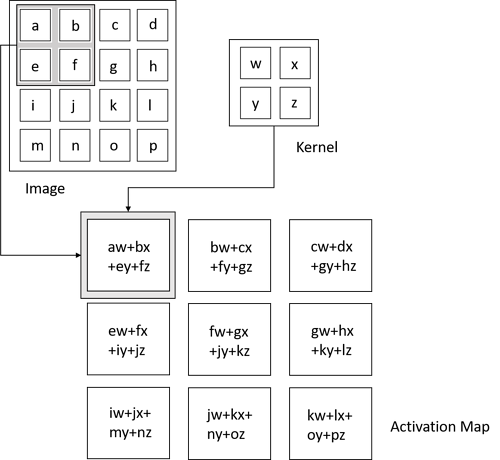
\includegraphics[scale=0.5]{Sources/CNN.png}
	\caption{Funktionsweise der Faltungsschicht \cite{convolutional2019layer}}
	\label{img:faltungsschicht}
\end{figure}\\
\textbf{Pooling Schicht}\\
Die Pooling Schicht oder auch \textit{Pooling Layer} kommt nach jeder Faltungsschicht \cite[336f.]{goodfellow2016deep}. Die Aufgabe dieser Schicht ist es das Eingabebild in der Auflösung und den zugehörigen Rechenaufwand für die folgenden Schichten zu reduzieren. Üblicherweise gibt es zwei Verfahren, welche beim Pooling eingesetzt werden. Zum einen das Average Pooling und das am häufigsten verwendete Max Pooling (Abb. \ref{img:maxpooling}). Auch diese Schicht besteht aus einem quadratischen Filter, welcher wie bei der Faltungsschicht über die Bildpunkte gelegt wird. Dabei wird beim \textit{Max Pooling} der höchste Wert in diesem Bereich ermittelt und übernommen. Bei einem standardmäßigem Kernel von 2x2, wird das Bild um den Faktor 2 Verkleinert. Die Abmessungen sind, anders wie bei der Faltungsschicht, gerade. 
\newpage
\begin{figure}
	[h]
	\centering
	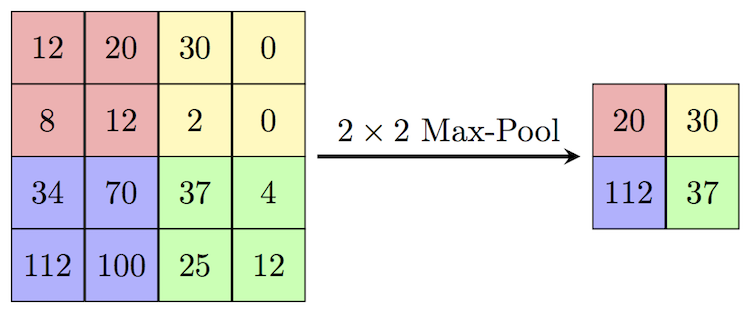
\includegraphics[scale=2.0]{Sources/MaxpoolSample2.png}
	\caption{Funktionsweise des Pooling Layers mit der Max Pooling variante \cite{pooling2018layer}}
	\label{img:maxpooling}
\end{figure}
\textbf{Fully Connected Layer}
nachdem das Eingabebild durch alle Faltungs- und Pooling Schichten verarbeitet wurde, werden die Daten an den Fully connected Layer übergeben \cite[14]{sermanet2012convolutional}. Dieser verwendet, wie bei einem normalen KNN, Perzeproten um die Daten zu verarbeiten. Die vorherigen Schichten wurden durchlaufen, damit diese rechenintensive Schicht nicht zu viel Informationen verarbeiten muss. 
  \subsubsection{Entstehung von Trainingsdaten}\label{s.trainingsdaten} 
Damit ein künstliches neuronales Netz Objekte erkennen und zuordnen kann, benötigt es zunächst eine Reihe von Beispieldaten. Anhand dieser Beispieldaten lernt das neuronale Netz, welche Eigenschaften das zu erlernende Objekt hat und wie es aufgebaut ist. Für diesen Vorgang werden üblicherweise mehrere Hunderttausend Daten benötigt, um ein akzeptables Ergebnis zu erzielen. Eine Möglichkeit, das Training mit weniger Trainingsdaten durchzuführen, ist das Verwenden vortrainierter Netze. Diese Netze wurden mit rund 300.000 Bildern über mehrere Tage trainiert und als Open Source zur Verfügung gestellt. Beim Verwenden dieser Netze werden lediglich die obersten Schichten, welche für die Zuweisung verantwortlich sind, durch den neuen Datensatz verändert wodurch wesentlich weniger Testdaten pro Objektklasse benötigt werden. 
\begin{figure}
	[h]
	\centering
	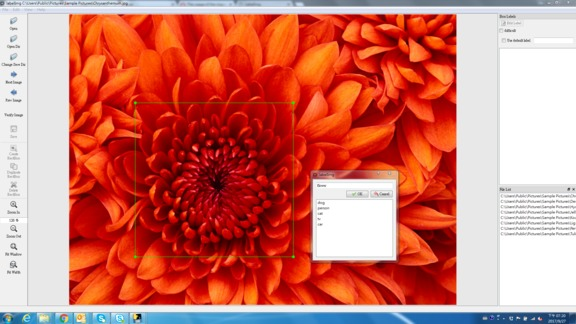
\includegraphics[scale=1.0]{Sources/labelimg.jpg}
	\caption{Vorbereitung der Datensätzen mit dem Labelimg Programm \cite{labelimg2019}}
	\label{img:labelimg}
\end{figure}\\
Eine Klassifizierung gehört zum überwachten Lernen und benötigt deswegen gelabelte Datensätze. Das Labeln wurde mit dem Open Source Programm \textit{LabelIMG} \cite{labelimg2019} durchgeführt. Dabei wird das zu Trainierende Objekt mit einem rechteckigen Kasten umschlossen und einer Klasse auf den Bildern markiert. Diese Daten werden zunächst in einer XML Datei abgespeichert. 
  \subsection{Mean average Precision}\label{s.map}
Oft können neuronale Netze nicht nur ein Objekt gleichzeitig erkennen, sondern geben als Ergebnis mehrere Hypothesen aus. Dadurch entsteht das Problem, das nicht mehr nur zwischen richtig und falsch unterschieden werden kann, sondern eine Genauigkeit benötigt wird, welche alle möglichen Objekte einbezieht. Eine Metrik welche auf diese Informationen eingeht, ist die (mean) average Precision (AP/mAP). Für die Berechnung wird die Präzision (Precision) und der Rückgabewert eines Ergebnisses benötigt. Die Präzision $P$ beschreibt den Anteil der richtig erkannten Objekte unter allen erkannten Objekten. Der Rückgabewert $R$ ist der korrekte Anteil von allen möglichen Objekten. Formell ausgedrückt:\\
\begin{eqnarray}
P&=&\frac{richtig\medspace erkannte}{richtig\medspace erkannte + falsch\medspace erkannte}\\
R&=&\frac{richtig\medspace erkannte}{richtig\medspace erkannte + falsche\medspace nicht\medspace erkannte}
\end{eqnarray}\\
Häufig wird ein Schwellwert für die Pseudowahrscheinlichkeit genutzt, mit welchem entschieden wird, wann ein erkanntes Objekt der Rückgabeliste hinzugefügt wird oder nicht. Wird der Schwellwert niedrig angesetzt, werden meist mehr Objekte, als erkannt eingestuft. Dadurch steigt der Rückgabewert mit richtig erkannten Objekten. Gleichzeitig sinkt aber auch die Präzision da natürlicherweise auch mehr falsche Objekte erkannt werden. Objekterkennungsverfahren mit einer hohen Qualität zeigen aber weiterhin eine gute Präzision.

\newpage
  \section{Methodik und Durchführung}\label{s.methudurchf}
Nach der theoretischen Grundlage soll sich der zweite Teil der Arbeit um die Versuchsbeschreibung, Durchführung und Auswertung der Ergebnisse handeln. Dabei werden zunächst die verwendeten Datensätze sowie die umsetzung der Normalisierungs Algorithmen. In den Ergebnissen, wird auf die Versuchsumgebung und die verwendeten Frameworks eingegangen, und wie diese für den Versuch genutzt wurden.
 \subsection{Verwendetes Modell}\label{s.modell}
Das Unternehmen COCO \cite{common2018data} (Common Objects in Contexts) besitzen eine vielzahl an Datensätzen mit welchen, neuronale Netze trainiert werden können. Einige dieser Netze wurde auf der Object detection API von Tensorflow trainiert und stehen als Open Source zur Verfügung. Die folgende Tabelle führt ausgewählte Modelle auf, um die Genauigkeit und Geschwindigkeit vergleichen zu können.\\
\begin{table}
[h]
\caption{Modelle \cite{google2018tens} welche mit dem COCO Dataset Trainiert wurden \cite{common2018data}}
\centering
\begin{tabular}{|l|c|c|}
\hline
Modell & mAP & Geschwindigkeit\\
\hline
faster\_rcnn\_inception\_v2\_coco & 28 & 58\\
faster\_rcnn\_resnet50\_coco & 30 & 89\\
rfcn\_resnet101\_coco & 30 & 92\\
ssd\_mobilenet\_v1\_coco & 30 & 21\\
ssd\_resnet\_50\_fpn\_coco & 35 & 76\\
\hline
\end{tabular}
\end{table}\\
Das faster\_rcnn\_inception\_v2\_coco soll für das Projekt verwendet werden. Dieses hat eine mAP von 28 und eine Geschwindigkeit von 32 ms. Dadurch das es die niedrigste mAP hat, sollten die Unterschiede in der Genauigkeit stärker ausfallen. Das ausgewählte Modell wird im folgenden auf die Datensätze, welche im anschließenden Unterkapitel aufgeführt sind.
  \subsection{Trainingsdaten}\label{s.tdaten}
  ??? Da für ein solches Training nicht die benötigten Ressourcen zur Verfügung stehen, sollte eine Möglichkeit gefunden werden, wie das Training auch mit weniger Trainingsdaten durchgeführt werden kann ??? Dieser Satz gehört zu durchführung nicht in den Theorewtischen teil???. Durch das vortrainieren werden nur noch durchschnittlich 150 Bilder pro Objektklasse und eine geringere Trainingszeit benötigt. Die Bilder der eigenen Daten werden mit einer normalen 12 Megapixel Kamera aufgenommen. Die verwendeten Objekte, müssen von allen möglichen Seiten fotografiert werden, dabei müssen, für das Training, pro klasse ungefähr 150 Bilder vorhanden sein. Da die Bilder mit einer 12 Megapixel Kamera mehrere 100 MB groß werden, müssen diese auf 100-200 KB komprimiert werden. ???\\

Damit am Ende des Projektes möglichst gute Vergleichswerte entstehen, werden mehrere Datensätze vor den Versuch verwendet. Insgesamt werden die neuronalen Netze mit 3 unterschiedlichen Datensätzen trainiert. Dafür wurden 3 Datensätze heraus gesucht. Der erste Datensatz welcher getestet wird, ist der Nahrungsmittel Datensatz eines früheren Projektes, zum anderen der Datensatz von \textit{Pascal Visual Object Classes} (PascalVOC) und der Hunderassen Datensatz, Stanford Dog Dataset.\\
In den folgenden Tabellen werden alle Datensätze mit den zugehörigen Klassen und Anzahl an Trainingsbildern aufgeführt:\\\\
Der erste Datensatz besteht aus mehreren Nahrungsmitteln, welche in der Tabelle \ref{tab:nahrungsmittel} jede klasse besitzt um die 100-150 Bilder welche zusätzlich Annotations-Dateien mit den Koordinaten der Klassifizierungsboxen beinhalten. Dieser Datensatz ist mit seinen ca. 1000 Bildern der kleinste Datensatz 
\begin{table}
[h]
\caption{Datensatz mit Nahrungsmitteln}
\centering
\begin{tabular}{|l|l|}
\hline
Klassenname & Klassenname\\
\hline
Milch - Packung & Orangensaft - Packung\\
Wasser - Flasche & Bier - Flasche\\
Brunch - Aufstrich & Margarine - Aufstrich\\
\hline
\end{tabular}
\label{tab:nahrungsmittel}
\end{table}\\
Der PascalVOC Datensatz umfasst 20 Klassen und besteht aus 5.000 Bildern. Von 2005 bis 2012 wurde jährlich die PascalVOC Challenges durchgeführt. Dabei sollte das beste verfahren für die Segmentierung, Klassifikation und Objekterkennung ermittelt werden. Inhaltlich befasst sich der Datensatz mit einer reihe unterschiedlicher Klassen, welche in Tabelle \ref{tab:pvoc} zu erkennen sind. Es gibt einige Unterschiede in der Häufigkeit der auftretenden Klassen. Beispielsweise sind in rund 2000 Bildern insgesamt 4.690 Personen enthalten, weswegen es möglicherweise Unterschiede in der Genauigkeit untereinander, der Klassen geben könnte. Die Aufnahmen der Bilder sind thematisch und und von der Art der Aufnahme unstrukturiert, was bedeutet, dass teilweise Bilder von einzelnen Objekten, Gruppen von Objekten oder auch ganze Szenen enthalten sind.\\
\begin{table}
[h]
\caption{Pascal Visual Object Classes \cite{pascal-voc-2007}}
\centering
\begin{tabular}{|l|l|l|l|}
\hline
Klassenname & Klassenname & Klassenname & Klassenname\\
\hline
Person & Vogel & Katze & Kuh\\
Hund & Pferd & Schaf & Zug\\
Flugzeug & Fahrrad & Boot & Bus\\
Auto & Motorrad & Flasche & Stuhl\\
Tisch & Blumentopf & Sofa & Bildschirm\\
\hline
\end{tabular}
\label{tab:pvoc}
\end{table}\\
Der dritte Datensatz welcher in dieser Arbeit verwendet wird, ist der Hunde Datensatz aus Stanford und beinhaltet 120 verschiedene Hunderassen. Jede Klasse hat um die 200 Bilddaten. Wegen der Struktur des Datensatzes, in einzelnen Ordnern, kann eine Auswahl der priorisierten Hunderassen zusammengestellt werden. Für den Versuch und damit eine bessere Übersicht erreicht werden kann, wurden 20 Hunderassen ausgewählt. Die Annotationen der Daten sind in Form von XML Dateien beigefügt. In der folgenden Tabelle werden die ausgewählten Klassen des Datensatzes zusammengefasst.\\
\begin{table}
[h]
\caption{Stanford Dog Dataset \cite{KhoslaYaoJayadevaprakashFeiFei_FGVC2011}}
\centering
\begin{tabular}{|l|l|l|l|}
\hline
Klassenname & Klassenname & Klassenname & Klassenname\\
\hline
Chihuahua & Japanese spaniel & Maltese dog & Pekinese\\
Shih-Tzu & Blenheim Spaniel & Papillon & Toy Terrier\\
Rhodesian Ridgeback & Afghan Hound & Basset & Beagle\\
Bloodhound & Bluetick & coonhound & Walker Hound\\
Redbone & Borzoi & Irish Wolfhound & Italian Greyhound\\
\hline
\end{tabular}
\end{table}\\
Von der Struktur der Datensätze, sind sie ähnlich aufgebaut. Viele verschiedene Klassen mit verschiedenen Szenen und Kontexten. Im weiteren wird zunächst auf die Umsetzung der Normalisierungsverfahren eingegangen, um weiter Erkenntnisse zu erlangen.
\newpage
\subsection{Normalisierung-Algorithmen}\label{s.nalgorithmen}
Für die Normalisierung der Datensätze ist eine Methode nötig, um mehrere Bilder möglichst schnell hintereinander zu bearbeiten. Für die Normalisierung wurden Python Programme geschrieben, welche nacheinander die Bilder, anhand eines Algorithmus verarbeitet. Dafür wurde mit unter die \textit{Python Image Libary} und OpenCV genutzt. Beide Bibliotheken werden für das verarbeiten von Bildern benötigt. 
\subsubsection{Gray-World-Algorithmus}
\begin{lstlisting}
# Importieren des Bildes
nimg = cv.imread(i, 1)

# Umwandlung des Bildes und der Kanäle in 32 Bit
nimg = nimg.transpose(2, 0, 1).astype(np.uint32)

# Zwischenspeichern des durchschnittlichen Grünkanals in die Variable mu_g
mu_g = np.average(nimg[1])

# Berechnng des rot-Kanals: 
nimg[0] = np.minimum(nimg[0]*(mu_g/np.average(nimg[0])),255)

# Berechnung des blau-Kanals:
nimg[2] = np.minimum(nimg[2]*(mu_g/np.average(nimg[2])),255)

Zurükwandlung des Bildes in 8 Bit
img_output = nimg.transpose(1, 2, 0).astype(np.uint8)
\end{lstlisting}
In dem verwendeten Gray World Algorithmus \cite{gray2012world} zunächst wird das Bild in 32 Bit umgewandelt. Daraufhin wird der Grünkanal verwendet und der Durchschnitt berechnet und zwischengespeichert. Der Grün-Kanal wird nun mit dem durchschnitt des Rot-Kanals dividiert. Das Ergebnis des wird mit dem Minimum des Rot-Kanals multipliziert und übernommen. Der gleiche Vorgang folgt mit dem Blau-Kanal. Das verarbeitete Bild wird nun wieder zurück in 8 Bit gewandelt und ausgegeben. Für das verfahren wird keine spezielle Python Bibliothek eingesetzt.
\begin{figure}
	[h]
	\centering
	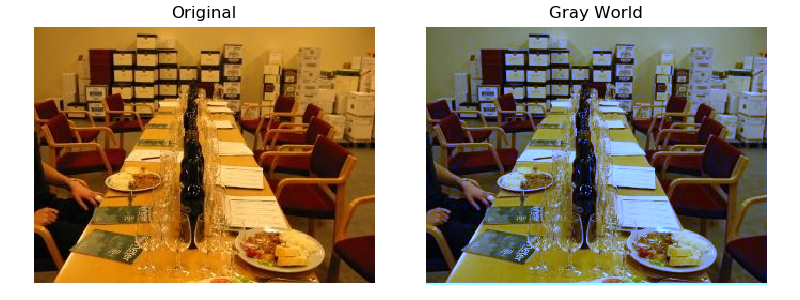
\includegraphics[scale=0.7]{Sources/gwn.png}
	\caption{Auswirkung des Gray-World Algorithmus}
	\label{img:gwnimg}
\end{figure}
\subsubsection{Histogramm Ausgleich}
\begin{lstlisting}
# Importieren des Bildes
img = cv2.imread('input.jpg')

# Umwandlung des Farbraumes von BGR zu YUV
img_yuv = cv2.cvtColor(img, cv2.COLOR_BGR2YUV)

# Ausgleichung vom Histogramm des Y Kanals
img_yuv[:,:,0] = cv2.equalizeHist(img_yuv[:,:,0])

# Umwandlung des Farbraumes in den BGR Farbraum
img_output = cv2.cvtColor(img_yuv, cv2.COLOR_YUV2BGR)
\end{lstlisting}
Für die Histogramm Ausgleichung \cite{histogram2012equalisation} wird das Bild zunächst vom BGR Farbraum in den YUV Farbraum umgewandelt. Der Farbraum ist ähnlich dem Lab Farbraum (Absch.\ref{s.lab}). Der Y Kanal wird für die Histogramm Ausgleichung verwendet. Das hat den Grund, dass das Luminanzsignal oder auch Leuchtdichte-Signal die Summe der drei Grundfarben Rot Grün und Blau und die Helligkeitsinformation enthält. Das Histogramm des Y Kanals wird, wie in Kapitel \ref{s.histogramme} beschrieben. Das normalisierte Bild wird von dem YUV Farbraum zurück in den BGR Farbraum konvertiert und zwischengespeichert. Das Ergebnis wird als Bild ausgegeben.
\begin{figure}
	[h]
	\centering
	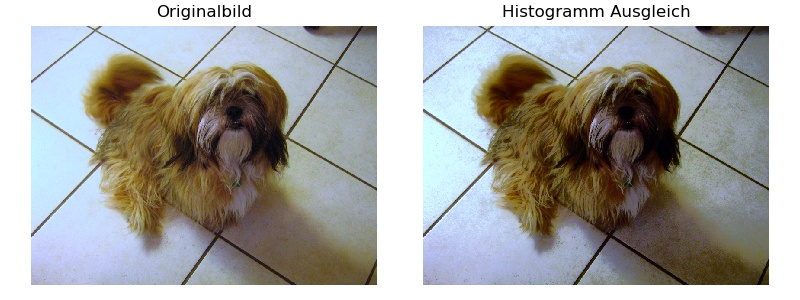
\includegraphics[scale=0.7]{Sources/histeq.jpg}
	\caption{Auswirkung der Histogramm Ausgleichung}
	\label{img:histogrameq}
\end{figure}
	
\subsubsection{Histogramm Spezifikation}
\begin{lstlisting}
# Importieren des Referenzbildes
reference = io.imread('reference.jpg')

# Importieren des zu Normalisierenden Bildes
image = io.imread('image.jpg')

# Weiterleitung der beiden Bilder an die match_histogram-Methode der Skimage Bibliothek
matched = match_histograms(image, reference, multichannel=True)
\end{lstlisting}
Der dritte Normalisierungsfunktion welche für die Datensätze angewendet wird, ist die Histogramm Spezifikation (Absch.\ref{s.hs}) oder auch \textit{Histogramm Matching}. Für den Algorithmus wird die Python Bibliothek \textit{Scikit-image} verwendet. Dafür werden ein Referenzbild und ein Zielbild geladen. Diese beiden Bilder, werden mit der Funktion \textit{match\_histograms} verarbeitet. Das Zielbild wurde auf das Histogramm des Referenzbildes angepasst. In dem Beispiel \ref{img:histogramspez} kann man gut erkennen, das das Quellbild, welches stark verdunkelt ist, durch ein gut ausgeleuchtetes Referenzbild, eine wesentlich bessere Helligkeit aufweist. Die Problematik bei dieser Normalisierungs Methode besteht darin, das ein einheitliches Referenzbild genutzt werden muss auf welchem dann der gesamte Datensatz Normalisiert wird.
\begin{figure}
	[h]
	\centering
	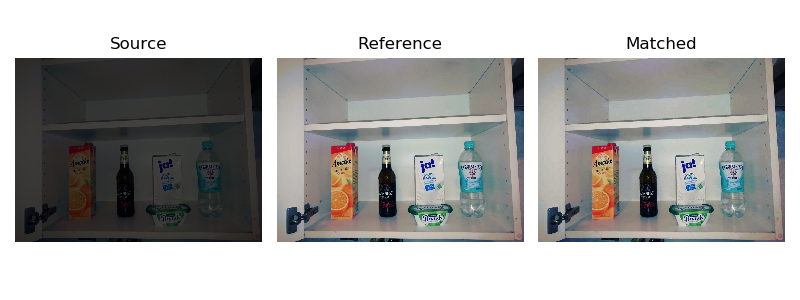
\includegraphics[scale=0.8]{Sources/HS_beispiel.png}
	\caption{Das Zielbild wurde mithilfe des Referenzbildes ausgeglichen und angepasst. Auf der linken Seite ist das Ergebnis der Spezifikation}
	\label{img:histogramspez}
\end{figure}
  \newpage
  \section{Ergebnisse}
Nachdem alle Trainingseinheiten mit den verschiedenen Normalisierungsverfahren durchlaufen wurden, sollen die Ergebnisse aufgeführt und verglichen werden. Zunächst wird auf die Entwicklungsumgebung beschrieben und im Anschluss auf die Ergebnisse der Auswertung. Als Vergleichswerte konnte mithilfe von Tensorboard die Genauigkeiten des Netzes erhoben werden. Jede Klasse hat eine eigene durchschnittliche Genauigkeit (AP) und eine Genauigkeit für das gesamte Netz in Form einer mAP. In den folgenden Tabellen werden bestimmte Abkürzungen verwendet: N = Normaler Datensatz, GW = Gray-World-Algorithmus, HA = Histogramm Ausgleich, HS = Histogramm Spezifikation (Die besten Ergebnisse einer Klasse wurden durch Fettschrift hervorgehoben) 
\subsection{Frameworks und Entwicklungsumgebung}\label{s.entwicklung}
Wie in vorherigen Kapiteln schon beschrieben ist das Trainieren eines künstlichen neuronalen Netzes oder eines faltenden neuronalen Netzes sehr rechenintensiv. Die enthaltenen Daten werden parallel mittels Matrizenmultiplikation verarbeitet. Aus diesem Grund werden für die Verarbeitung Grafikprozessoren hauptsächlich verwendet da diese im Gegensatz zu normalen Prozessoren für die Berechnung von Matrizen konzipiert wurden.\\
Auf Softwareseite gibt es eine Menge an Frameworks, mit welcher sich CNNs realisieren lassen. Einige von denen sind beispielsweise Tensorflow, Keras und Theano. Wegen der vorliegenden Erfahrung und der Möglichkeit Trainingsfortschritte grafisch anzeigen zu können, wird der praktische Teil der Arbeit mittels Tensorflow durchgeführt. Tensorflow ist ein Open Source Framework von Google, welches zum entwickeln künstlicher neuronaler Netze genutzt werden kann. Programmiert wurde das Framework in den Programmiersprachen C und Python, welche auch für die Entwicklung genutzt werden. Mit dem Framework Tensorflow kommen einige Möglichkeiten. Zum einen gibt es eine übersichtliche Dokumentation, zum anderen werden vortrainierte Netze, Open Source und für die Entwicklung die Tensorflow Object Detection API angeboten. Zur Verfügung stehen verschiedenste Netze auf Basis von verschiedenen Datensätzen.
  \subsection{Nahrungsmittel Datensatz}
Der erste Datensatz welcher untersucht wurde ist der Datensatz, welcher in der Tabelle \ref{tab:nahrungsmitteltest} aufgeführt ist. Dieser enthält im Vergleich zu den anderen Datensätzen weniger Objektklassen und weniger Bilder. Außerdem ist, sind die Objekte unter ähnlichen Bedingungen entstanden. Das bedeutet, dass die Lichteinstrahlung in den meisten Fällen gleich ist und nur auf wenigen unterschiedlichen Hintergründen aufgenommen wurden. In der Tabelle \ref{tab:nahrungsmitteltest} wurde der Nahrungsmittel Datensatz verwendet und enthält die Informationen des originalen Datensatzes, des Gray-World Algorithmus, des Histogramm Ausgleichs und der Histogramm Spezifizierung. Im genauen Betrachten fällt auf, dass kaum nennenswerte Unterschiede bei GW entstanden sind. In manchen Punkten können Verbesserungen in der Genauigkeit ausgewertet werden(Wasser, Orangensaft, Bier), in anderen wiederum ist die Genauigkeit gesunken(Milch, Brunch, mAP).\\
Bei den Histogramm Normalisierungen (Ausgleich und Spezifizierung) kann mehr interpretiert werden. Auch hier sind die Unterschiede nur in einzelnen Objektklassen besser geworden und in anderen zurückgegangen. Die Varianz der verschiedenen Netze liegt bei gerade mal 0.05, was in der Praxis keinen bedeutenden Unterschied macht. Dennoch schneiden die Histogramm Normalisierungen insgesamt am schlechtesten ab.
\begin{table}
[h]
\caption{Durchschnittliche Genauigkeiten des Modells mit dem Nahrungsmittel Datensatz}
\centering
\begin{tabular}{|l|c|c|c|c|}
\hline
Klassenname & AP(N) & AP(GW) & AP(HA) & AP(HS)\\
\hline
Wasser - Flasche & 0.948 & \textcolor{green}{0.955} & 0.934 & \textcolor{red}{0.917}\\
Orangensaft - Packung & 0.999 & \textcolor{red}{0.998} & \textcolor{green}{1.000} & 0.999\\
Milch - Packung & \textcolor{green}{1.000} & \textcolor{green}{1.000} & \textcolor{green}{1.000} & \textcolor{green}{1.000}\\
Margariene & \textcolor{green}{1.000} & \textcolor{green}{1.000} & \textcolor{green}{1.000} & \textcolor{green}{1.000}\\
Brunch - Aufstrich & \textcolor{green}{1.000} & 0.995 & \textcolor{red}{0.959} & 0.975\\
Flasche - Bier & \textcolor{green}{0.997} & \textcolor{red}{0.970} & 0.986 & 0.979\\
\hline
mAP & \textcolor{green}{0.991} & 0.987 & 0.980 & \textcolor{red}{0.978}\\
\hline
\end{tabular}
\label{tab:nahrungsmitteltest}
\end{table}
\subsection{PascalVOC Datensatz}
Beim Auswerten der Genauigkeit des normalen Modells fällt auf, das teilweise große Unterschiede der einzelnen Objektklassen auftreten. Das kann daher resultieren, dass unterschiedlich viele Bilder pro klasse enthalten sind. Ähnlich wie beim vorherigen Datensatz konnte zwischen dem originalen Datensatz und der Gray-World-Normalisierung kein deutlicher Unterschied festgestellt werden. Einige Klassen haben zwar eine höhere durchschnittliche Wahrscheinlichkeit, dennoch gibt es auch hier mehrere Bereiche, wo die Genauigkeit abgenommen hat. Auch die mAP hat ca. 0.8\% Genauigkeit verloren. Anders als beim Nahrungsmittel Datensatz schneidet der Histogramm Ausgleich schlechter ab. Nur ein paar Objektklassen konnten besser erkannt werden. Insgesamt verliert das neuronale Netz 3.4\% der Genauigkeit, was einen wichtigen Unterschied macht. Einige Objektklassen sinken durch die Ausgleichung unter die 50\% Genauigkeit, was vergleichbar mit raten wäre. Hier wird auch die Schwäche der Histogramm Spezifikation deutlich. Durchschnittlich 4.5\% Genauigkeit wird durch die Normalisierung eingebüßt. 
\begin{table}
[h]
\caption{Durchschnittliche Genauigkeiten des Modells mit dem PascalVOC Datensatz}
\centering
\begin{tabular}{|l|c|c|c|c|}
\hline
Klassenname & AP(N) & AP(GW) & AP(HA) & AP(HS)\\
\hline
sofa & 0.611 & 0.612 & \textcolor{green}{0.637} & \textcolor{red}{0.602}\\ 
aeroplane & 0.845 & \textcolor{green}{0.855} & \textcolor{red}{0.826} & 0.843\\
horse & \textcolor{green}{0.924} & 0.910 & \textcolor{red}{0.891} & 0.905\\
train & 0.790 & \textcolor{green}{0.804} & \textcolor{red}{0.797} & 0.817\\
bird & \textcolor{green}{0.750} & 0.733 & \textcolor{red}{0.691} & 0.708\\ 
tvmonitor & 0.729 & \textcolor{green}{0.733} & 0.725 & \textcolor{red}{0.691}\\
boat & \textcolor{green}{0.680} & 0.644 & 0.626 & \textcolor{red}{0.559}\\
pottedplant & \textcolor{green}{0.430} & 0.415 & 0.425 & \textcolor{red}{0.340}\\
bus & 0.797 & \textcolor{green}{0.810} & \textcolor{red}{0.763} & 0.776\\ 
diningtable & 0.532 & \textcolor{green}{0.545} & \textcolor{red}{0.507} & 0.517\\
car & 0.812 & \textcolor{green}{0.815} & 0.789 & \textcolor{red}{0.775}\\
bottle & \textcolor{green}{0.553} & 0.510 & 0.498 & \textcolor{red}{0.451}\\
cat & \textcolor{green}{0.903} & 0.902 & 0.872 & \textcolor{red}{0.841}\\
person & \textcolor{green}{0.791} & 0.779 & 0.775 & \textcolor{red}{0.757}\\
chair & 0.499 & \textcolor{green}{0.515} & 0.460 & \textcolor{red}{0.440}\\
bicycle & 0.744 & 0.730 & \textcolor{green}{0.752} & \textcolor{red}{0.697}\\
cow & \textcolor{green}{0.718} & 0.698 & 0.694 & \textcolor{red}{0.653}\\
motorbike & \textcolor{green}{0.739} & \textcolor{red}{0.722} & 0.725 & 0.725\\
dog & \textcolor{green}{0.867} & 0.862 & 0.835 & \textcolor{red}{0.811}\\
sheep & 0.645 & 0.619 & \textcolor{green}{0.664} & \textcolor{red}{0.561}\\
\hline
mAP & \textcolor{green}{0.718} & 0.710 & 0.698 & \textcolor{red}{0.673}\\
\hline
\end{tabular}
\end{table}
  \subsection{Stanford Dogs Dataset}
Auch bei Überprüfung des dritten Datensatzes fallen ähnliche Muster auf. Der GW-Algorithmus weißt bei diesem Datensatz sogar bessere Ergebnisse wie der originale Datensatz auf. Beim vergleichen der Datensätze fällt hier auf, das mehr verschiedene Lichtfarben genutzt wurden, als bei den anderen beiden Datensätzen. Diese konnten vom GW-Algorithmus vereinheitlicht werden. Beim Histogramm Ausgleich und der Spezifikation wurden wie auch bei den vorherigen Datensätzen schlechtere Genauigkeiten beobachtet.   
\begin{table}
[h]
\caption{Durchschnittliche Genauigkeiten des Modells mit dem Stanford Dog Datensatz}
\centering
\begin{tabular}{|l|c|c|c|c|}
\hline
Objektklasse & AP(N) & AP(GW) & AP(HA) & AP(HS)\\
\hline
Chihuaua & \textcolor{red}{0.729} & \textcolor{green}{0.854} & 0.780 & 0.746\\ 
Shih-Tzu & 0.864 & \textcolor{green}{0.879} & 0.857 & \textcolor{red}{0.832}\\
Rhodesian Ridgeback & \textcolor{green}{0.741} & 0.706 & 0.711 & \textcolor{red}{0.699}\\
Bloodhound & 0.872 & \textcolor{green}{0.878} & 0.904 & \textcolor{red}{0.848}\\
Redbone & \textcolor{green}{0.617} & 0.546 & \textcolor{red}{0.486} & 0.507\\ 
Japanese Spaniel & 0.886 & 0.919 & \textcolor{green}{0.939} & \textcolor{red}{0.837}\\
Blenheim Spaniel & \textcolor{green}{0.980} & 0.966 & 0.944 & \textcolor{red}{0.906}\\
Afghan Hound & \textcolor{green}{0.955} & \textcolor{red}{0.946} & 0.947 & 0.953\\
Bluetrick & \textcolor{green}{0.897} & 0.892 & \textcolor{red}{0.864} & 0.870\\ 
Borzoi & \textcolor{green}{0.931} & \textcolor{red}{0.922} & 0.932 & 0.925\\
Maltese dog & \textcolor{green}{0.905} & 0.901 & \textcolor{red}{0.874} & 0.784\\
Papillon & 0.971 & \textcolor{green}{0.984} & 0.973 & \textcolor{red}{0.952}\\
Basset & 0.763 & \textcolor{green}{0.779} & \textcolor{red}{0.707} & 0.711\\
Coonhound & \textcolor{red}{0.863} & 0.864 & \textcolor{green}{0.895} & 0.901\\
Irish Wolfhound & \textcolor{green}{0.945} & 0.930 & 0.940 & \textcolor{red}{0.905}\\
Pekinese & \textcolor{red}{0.723} & \textcolor{green}{0.840} & 0.743 & 0.782\\
Toy Terrier & 0.838 & \textcolor{green}{0.856} & \textcolor{red}{0.784} & 0.804\\
Beagle & 0.725 & \textcolor{green}{0.743} & \textcolor{red}{0.665} & 0.669\\
Walker Hound & \textcolor{green}{0.767} & \textcolor{red}{0.705} & 0.757 & 0.733\\
Italian Greyhound & 0.822 & \textcolor{green}{0.845} & 0.800 & \textcolor{red}{0.785}\\
\hline
mAP & 0.840 & \textcolor{green}{0.848} & 0.829 & \textcolor{red}{0.807}\\
\hline
\end{tabular}
\end{table}
\subsection{Zwischenstand}
Um herauszufinden wodurch die abnehmende Genauigkeit in der Klassifizierung entstanden ist, wurden die Trainingsdaten überprüft. Dabei ist aufgefallen das bei der Histogramm Ausgleichung und der Spezifikation große Unterschiede in den Datensätzen zu erkennen sind. Das liegt daran, das die Normalisierung die Farbinformationen des gesamten Bildes nimmt und diese anpasst. Dabei spielt es einen Unterschied, ob die Umgebung in dem Bild Hell, dunkel oder eine dominante Farbe haben. Bei der Histogramm Spezifikation kommt zusätzlich noch das Referenzbild hinzu welches für den Datensatz verwendet wird. Bei der Verwendeten Art von Datensätzen, wurde keine einheitliche Umgebung genutzt, sondern fast ausschließlich unterschiedliche. Durch diese unterschiedlichen Trainingsbildern kommt es zu Anomalien in den Normalisierten Bildern (Abbildung \ref{img:evalHA}). Ein Datensatz mit einheitlichem Hintergrund in den Trainingsdaten, könnte mit den Normalisierungs Verfahren besser funktionieren. Um diese Annahme weiter überprüfen zu können, soll ein weiterer Datensatz generiert werden, in welchem ein konstanter Hintergrund festgelegt ist.
\subsection{Obst Datensatz}
Für einen weiteren Versuch, wurde der Obstdatensatz erstellt. Dieser besteht aus den Objekten welche in Tabelle \ref{tab:obst} aufgelistet sind. Bei diesem Datensatz wurde darauf geachtet einen einheitlichen Hintergrund zu verwenden, um die Funktionalität bei anderen Einstellungen zu testen. Außerdem wurde im Vergleich zum Nahrungsmittel Datensatz (Tabelle.\ref{tab:nahrungsmittel}) darauf geachtet, ähnlichere Kassen zu verwenden, auf welchen optimaler Weise keine Schrift enthalten ist.
\begin{table}[htpb]
\caption{Klassen des Obst Datensatzes mit konstantem Hintergrund}
\begin{minipage}[r]{.5\textwidth} 
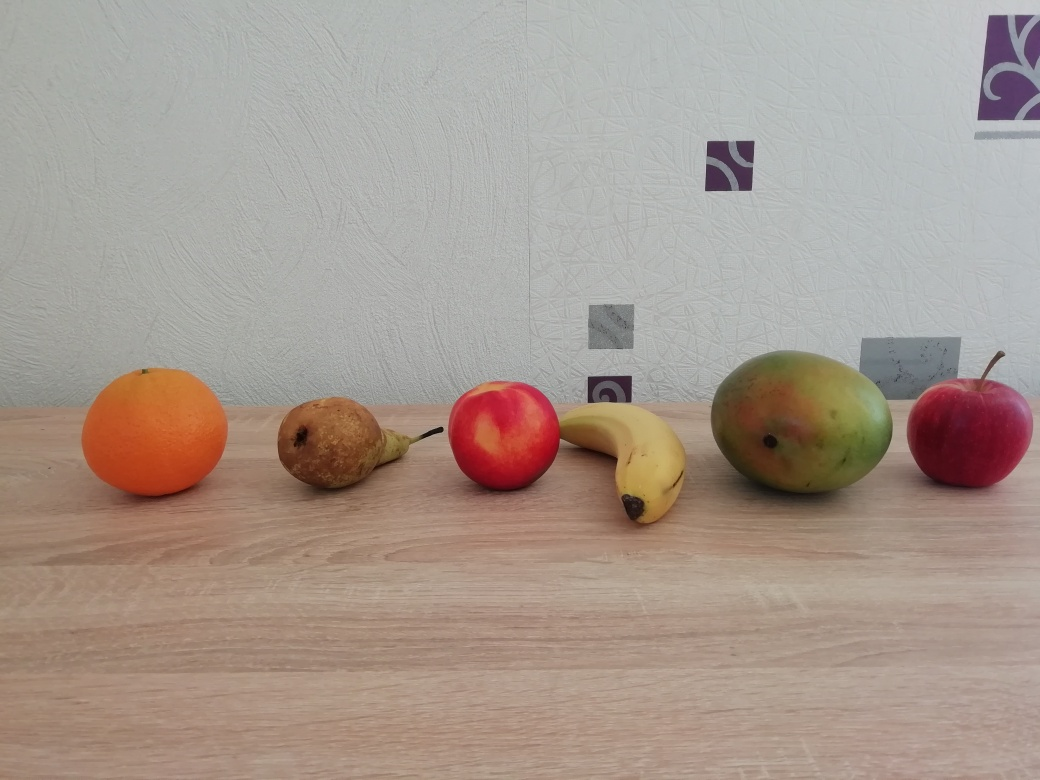
\includegraphics[width=.7\textwidth]{Sources/Obst_mit_hintergrund}  
\end{minipage} 
\hfill
\begin{minipage}[c]{.5\textwidth}\label{tab:obst} 
\centering  
\begin{tabular}{|l|l|}
\hline
Klassenname & Klassenname\\
\hline
Orange & Mango\\
Banane & Nektarine\\
Apfel & Birne\\
\hline
\end{tabular} 
\end{minipage}
\end{table}  
Dieser Datensatz wird nun genau wie die vorherigen Datensätze, mit den unterschiedlichen Methoden Normalisiert. Dabei soll zum einen die Genauigkeit der einzelnen Klassen betrachtet werden, zum anderen die Trainingsdaten an sich. Dabei soll überprüft werden, ob die Trainingsbilder wie erwartet aussehen und was für Anomalien auftreten. 
\subsection{Auswertung des Obst Datensatzes}
Nach Auswertung der Trainingsergebnisse kann festgestellt werden, das die Normalisierungsmethoden keinen Negativen Einfluss auf den Datensatz haben. Da die genauigkeit bei 100\% der Testdaten lagen, kann von den Zahlen aus, leider keine Aussage getroffen werden, inwieweit die Methoden einen positiven Einfluss auf die Klassifizierung haben. Eine weitere Möglichkeit dies zu überprüfen, könnte mit Hilfe besonders schwierigen Testbildern überprüft werden. Dafür sollen Bildaufnahmen bei sehr unterschiedlichen Lichteinflüssen verwendet werden.
\begin{table}
[h]
\caption{Genauigkeits-Berechnungen des Modells des Obst Datensatzes}
\centering
\begin{tabular}{|l|c|c|c|c|}
\hline
Klassenname & AP(N) & AP(GW) & AP(HA) & AP(HS)\\
\hline
Orange & 1.000 & 1.000 & 1.000 & 1.000\\
Nektarine & 1.000 & 1.000 & 1.000 & 1.000\\
Banane & 1.000 & 1.000 & 1.000 & 1.000\\
Mango & 1.000 & 1.000 & 1.000 & 1.000\\
Apfel & 1.000 & 1.000 & 0.999 & 1.000\\
Birne & 1.000 & 1.000 & 1.000 & 1.000\\
\hline
mAP & 1.000 & 1.000 & 1.000 & 1.000\\
\hline
\end{tabular}
\end{table}\\
Die Auswertung der normalisierten Trainingsdaten hat ergeben, das wesentlich weniger farb-Anomalien auftreten. Dabei ist aufgefallen das gerade bei den Histogramm Normalisierungen mit einheitlichen Hintergrund deutliche Verbesserungen erzielt wurden. Zu große Veränderungen treten nur dann auf, wenn viele Objekte auf dem Bild enthalten sind, da diese die Umgebung zu stark beeinflussen oder wenn die Beleuchtungen zu extrem verändert werden. Die Histogramm Spezifikation geht mit diesem Problem noch am besten um, weil dieser ein Referenz-Histogramm hat, um es anzupassen. \\\\
Auch eine Betrachtung der Helligkeitsverteilung der Trainingsdaten werden wesentlich besser wie in den Beispielen in Abbildung \ref{img:hellver} zu erkennen ist. Dafür wurde eine stark unterbelichtete Aufnahme generiert, um die Veränderung nach den Normalisierungs Methoden besser herauszustellen. Die beste Helligkeitsverteilung konnte dabei der Histogramm Ausgleich aufweisen, wobei durch das dunkle Quellbild die Farbinformationen zum großen Teil verloren gegangen sind. Der Gray World hat die Helligkeitsverteilung kaum verändert, was aber daran liegt, das die Farbverteilung durch die Höhe des Grün Kanals verschoben wird und nicht für solche Aufgaben ausgelegt ist. Das insgesamt beste Ergebnis liefert die Histogramm Spezifikation. Nicht nur die Helligkeitsverteilung konnte verbessert werden, auch die Farben konnten vergleichsweise gut wieder hergestellt werden.
  \newpage
\section{Diskussion}
In diesem Kapitel sollen die Ergebnisse und Erkenntnisse welche im Verlauf der Arbeit herausgearbeitet wurden kurz aufgeführt und erläutert werden, damit am ende ein Gesammtfazit gezogen werden kann.\\\\
Die Ergebnisse der trainierten Netze zeigen, dass mit die verwendeten Datensätzen zusammen mit den angewandten Normalisierungsmethoden keine Erhöhung der Genauigkeit erzielen. Ein möglicher Grund könnte zum einen in den vortrainierten Netzen liegen, welche schon zu genau und hochwertig eingestellte Perzeptronen besitzen und durch die vorherigen Datensätze nicht optimal für den Versuch waren. Zum anderen könnte es an den Datensätzen selber liegen, welche normalisiert wurden. Dafür wurden Objekte mit gleicher Lichteinstrahlung und gleicher Entfernung auf unterschiedlichen Hintergründen aufgenommen. Das Objekt wurde vom Hintergrund segmentiert, um zu überprüfen, wie sich die Histogramme voneinander unterscheiden (Abb.\ref{img:evalnorm}). Dieser Vorgang wurde daraufhin auch mit der Histogramm Ausgleichung überprüft (Abb.\ref{img:evalHA}).\\
\begin{figure}[htb]
\begin{minipage}[c]{0.2\textwidth}
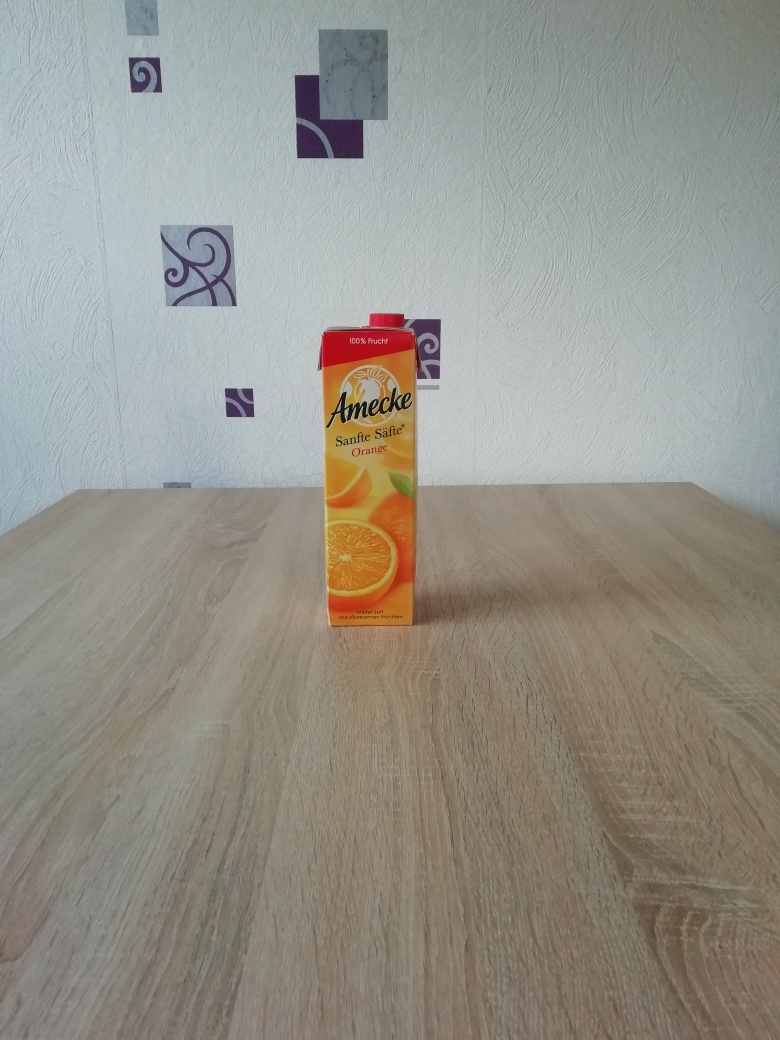
\includegraphics[width=\textwidth]{Sources/Bild1.jpg}
\end{minipage}
\hfill
\begin{minipage}[c]{0.08\textwidth}
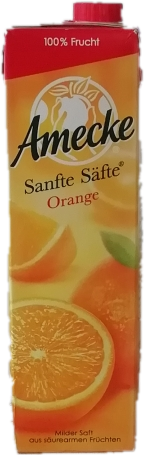
\includegraphics[width=\textwidth]{Sources/Bild1.png}
\end{minipage}
\hfill
\begin{minipage}[c]{0.3\textwidth}
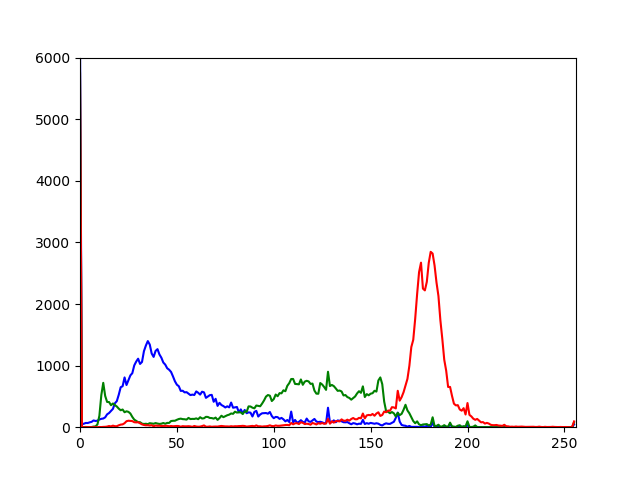
\includegraphics[width=\textwidth]{Sources/Bild1_histo.png}
\end{minipage}
\end{figure}
\begin{figure}[htb]
\begin{minipage}[c]{0.2\textwidth}
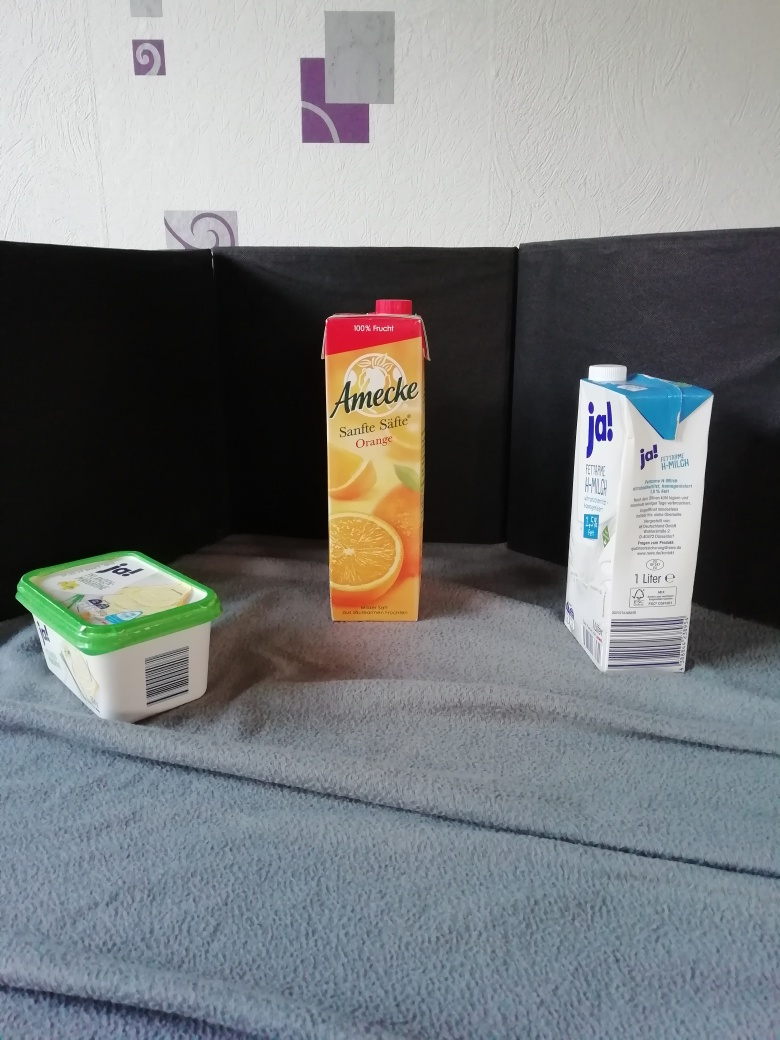
\includegraphics[width=\textwidth]{Sources/Bild2.jpg}
\end{minipage}
\hfill
\begin{minipage}[c]{0.08\textwidth}
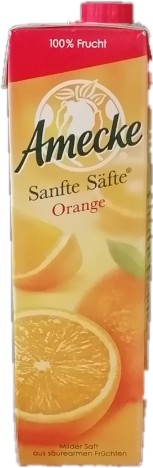
\includegraphics[width=\textwidth]{Sources/Bild2.png}
\end{minipage}
\hfill
\begin{minipage}[c]{0.3\textwidth}
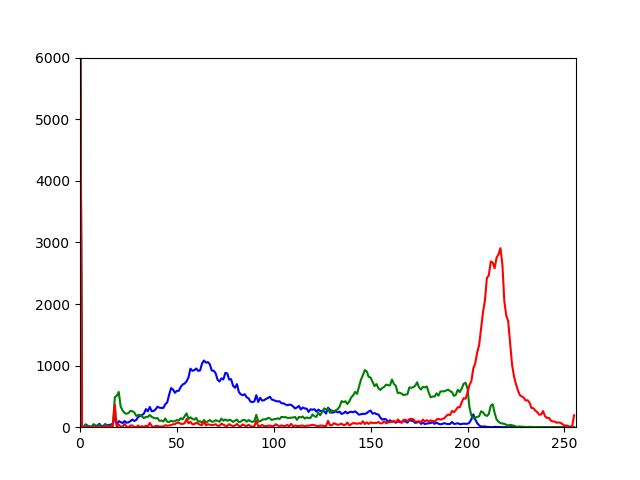
\includegraphics[width=\textwidth]{Sources/Bild2_histo.png}
\end{minipage}
\caption{Histogramm des Segmentierten Objektes aus dem Nahrungsmittel Datensatz. Ohne Normalisierung}
\label{img:evalnorm}
\end{figure}\\
Bei den normalen Datensätzen ist aufgefallen, das bei gleicher Lichteinstrahlung und unterschiedlichen Hintergründen die Objekte eine unterschiedliche Farbverteilung aufweisen. Das könnte durch Lichtreflexionen anderer Objekte in der Umgebung erklärt werden. Der normalisierte Datensatz weißt sogar noch größere Unterschiede in den Klassen auf. Das liegt daran, dass die Normalisierung nicht nur die Objekte auf den Bildern normalisiert, sondern auch den Hintergrund, welcher bei vielen Bildern unterschiedlich ist, verrechnet. Das bedeutet, dass nicht der Datensatz untereinander normalisiert wurde, sondern jedes Bild in dem Datensatz für sich.\\\\
Die Datensätze sind mit dem verwendeten Aufbau und den Normalisierungs Algorithmen nicht gut geeignet. Die Kriterien für einen Datensatz welcher durch Farbnormalisierung eine höhere Genauigkeit erreichen könnte, liegt in dem Hintergrund, welcher verwendet wird. Dabei müssen alle Klassen mit demselben Hintergrund aufgenommen werden. Dadurch würden alle Klassen auf derselben Basis normalisiert werden. Gerade die Histogramm Spezifikation (Absch. \ref{s.hs}) hätte hier ein großes Potenzial, da die Auswahl eines Referenzbildes einfacher und effektiver wird, durch den einheitlichen Hintergrund. Um diese Theorie zu überprüfen, wird ein weiterer Datensatz generiert und gelabelt. 
\subsection{Laufzeittest}
Ein weiterer Einfluss welches die Normalisierungs Algorithmen auf die Klassifizierung von neuronalen Netzen haben, ist neben dem Manipulieren von Trainingsdaten, die Zeit welches die jeweiligen Verfahren benötigen. Um einen Eindruck zu bekommen, wurde Ein Bild in verschiedenen Größen getestet, um herauszufinden wie sich die Laufzeit bei größer werdenden Bilddateien verhält.
\begin{table}
[h]
\caption{Laufzeiten der Normalisierungs-Algorithmen mit verschieden großen Bildern}
\centering
\begin{tabular}{|l|c|c|c|c|c|}
\hline
Bildgröße & Faktor & Dateigröße & GW & HA & HS\\
\hline
4160x3120 & 100\% & 2.441 KB & 1,447s & 0,172s & 6,952s\\
2912x2184 & 70\% & 1.000 KB & 0,755s & 0,078s & 3,215s\\
2080x1560 & 50\% & 529 KB & 0,362s & 0,035s & 1,717s\\
1040x780 & 25\% & 114 KB & 0,094s & 0,013s & 0,422s\\
\hline
\end{tabular}
\end{table}
Der Gray World Algorithmus ist im Vergleich zu den anderen Methoden in der Mitte von der Laufzeit bei Verdoppelung der Bildgröße, erhöht sich die Laufzeit um das vierfache. Dabei ist auch die Farbgebung und der Kontrast nicht entscheidend. Die Histogramm Ausgleichung ist in diesem Fall die Schnellste Methode, wobei dafür die Verteilung im Histogramm eine Rolle spielt. Die Laufzeit verändert sich nicht Linear, sondern steigt exponential an. So steigt die Laufzeit beim verdoppeln um den Faktor drei, und beim nächsten mal um den Faktor sechs. Der längste Normalisierungs Algorithmus ist in diesem Fall die Histogramm Spezifikation. Dabei spielt die Größe des Referenzbildes eine wichtige Rolle. Mit einem größeren Referenzbild, würde sich die Laufzeit noch weiter erhöhen. Bei gleich bleibenden Referenzbild erhöht sich die Laufzeit um den Faktor vier. Durch die hohe Grunddauer führt das schnell zu langen Laufzeiten.\\\\
Dabei muss beachtet werden, das die Laufzeiten nur für ein Bild berechnet wurden. Für ein künstliches neuronales Netz werden meist mehrere Tausend Bilder verwendet. Hier muss, je nach Datensatz, abgewägt werden, ob eine Normalisierung für die erhöhte Laufzeit in Kauf genommen werden soll.   
  \section{Fazit}
  \newpage
  \printbibliography
  \newpage
  \section*{Anhang}
\begin{figure}[htb]
\begin{minipage}[c]{0.2\textwidth}
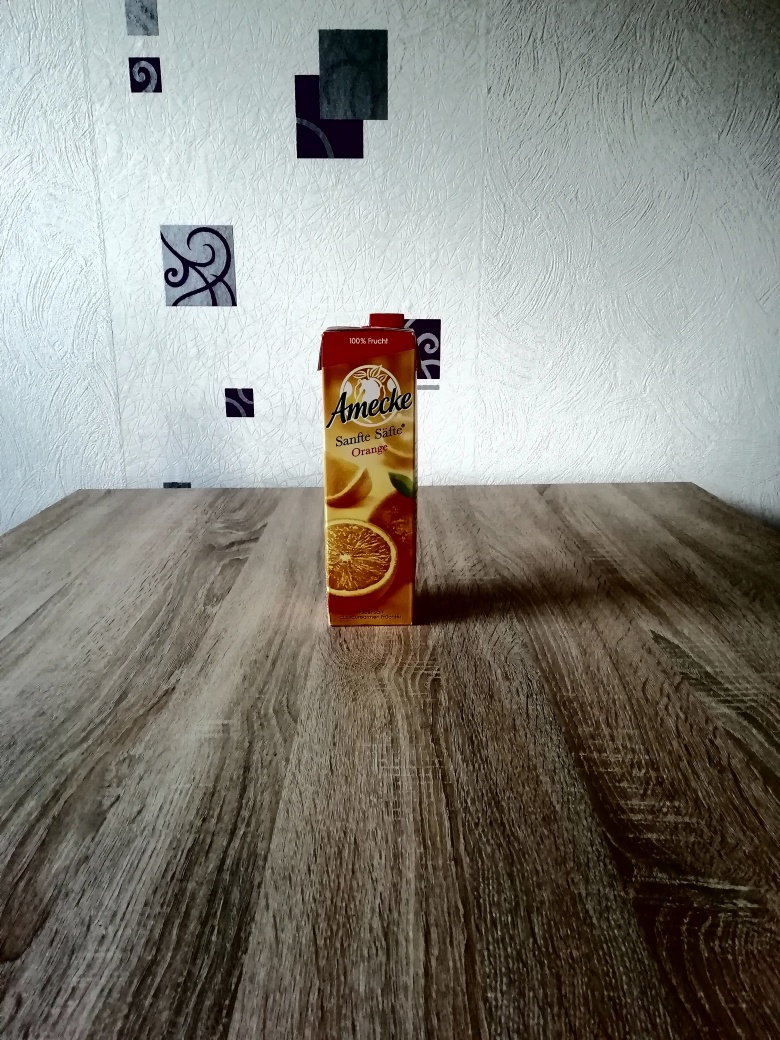
\includegraphics[width=\textwidth]{Sources/Bild1_HA.jpg}
\end{minipage}
\hfill
\begin{minipage}[c]{0.08\textwidth}
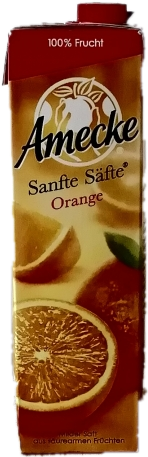
\includegraphics[width=\textwidth]{Sources/Bild1_HA.png}
\end{minipage}
\hfill
\begin{minipage}[c]{0.3\textwidth}
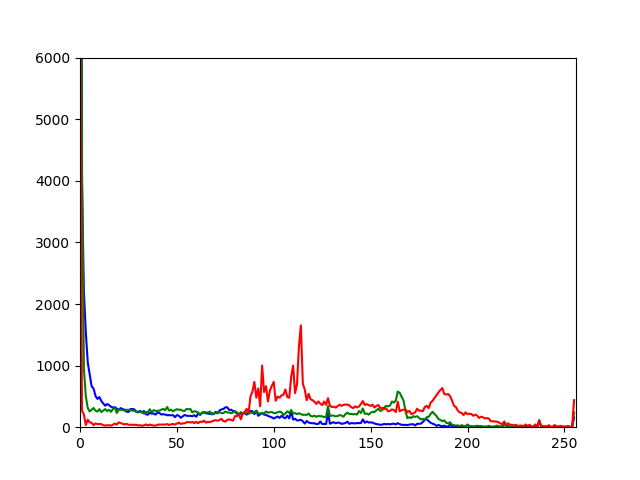
\includegraphics[width=\textwidth]{Sources/Bild1_HA_histo.png}
\end{minipage}
\end{figure}
\begin{figure}[htb]
\begin{minipage}[c]{0.2\textwidth}
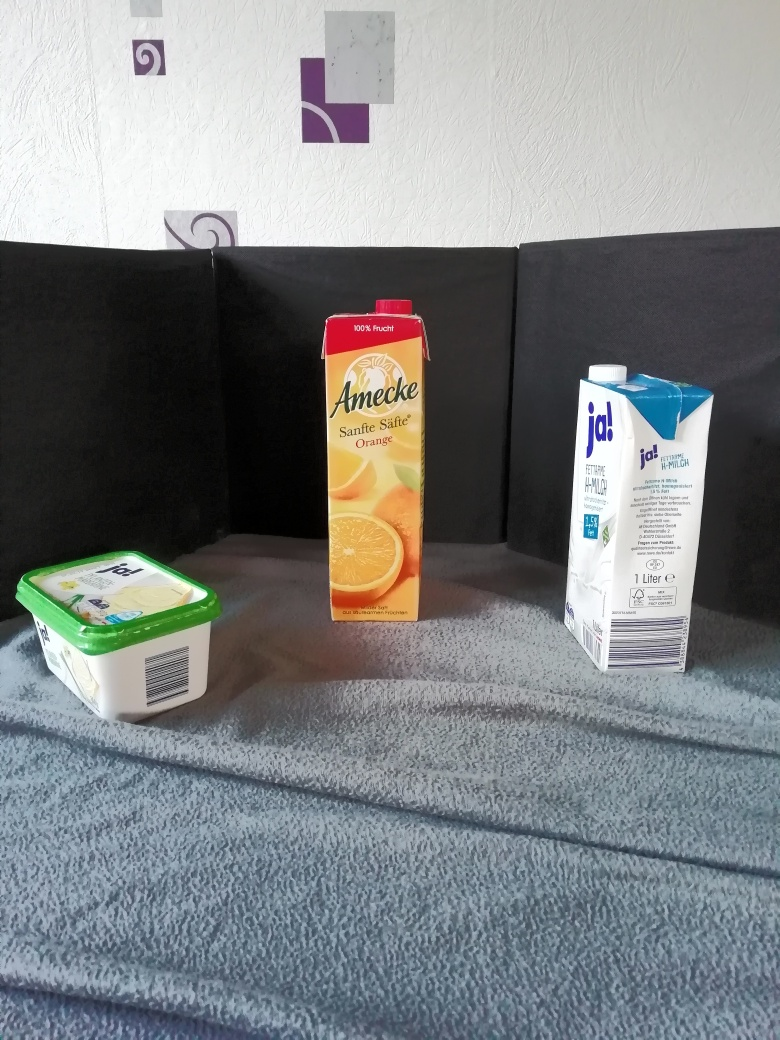
\includegraphics[width=\textwidth]{Sources/Bild2_HA.jpg}
\end{minipage}
\hfill
\begin{minipage}[c]{0.08\textwidth}
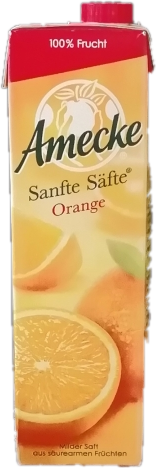
\includegraphics[width=\textwidth]{Sources/Bild2_HA.png}
\end{minipage}
\hfill
\begin{minipage}[c]{0.3\textwidth}
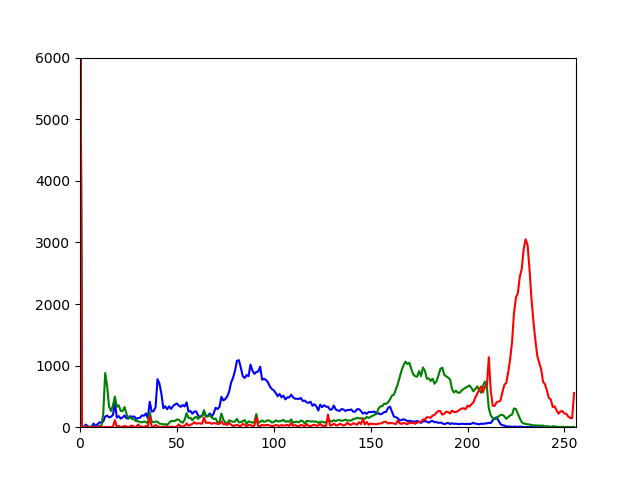
\includegraphics[width=\textwidth]{Sources/Bild2_HA_histo.png}
\end{minipage}
\end{figure}
\begin{figure}[htb]
\begin{minipage}[c]{0.2\textwidth}
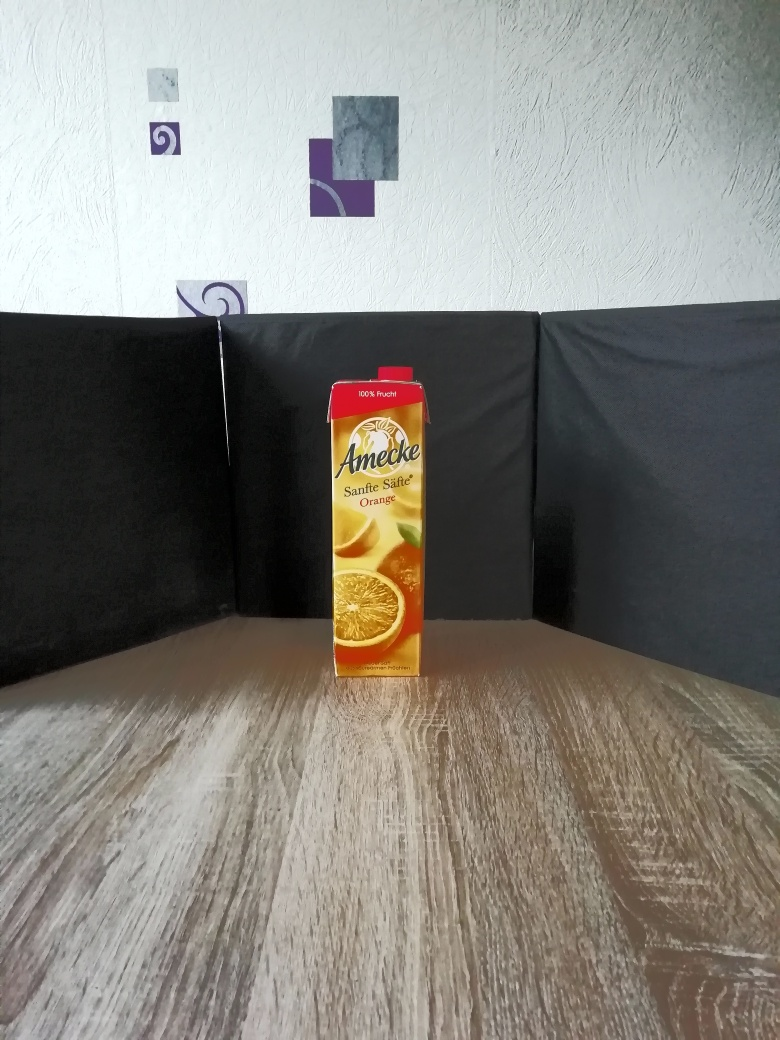
\includegraphics[width=\textwidth]{Sources/Bild3_HA.jpg}
\end{minipage}
\hfill
\begin{minipage}[c]{0.08\textwidth}
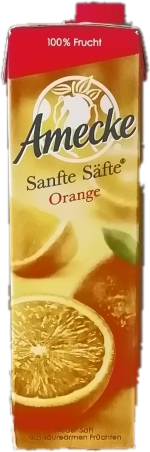
\includegraphics[width=\textwidth]{Sources/Bild3_HA.png}
\end{minipage}
\hfill
\begin{minipage}[c]{0.3\textwidth}
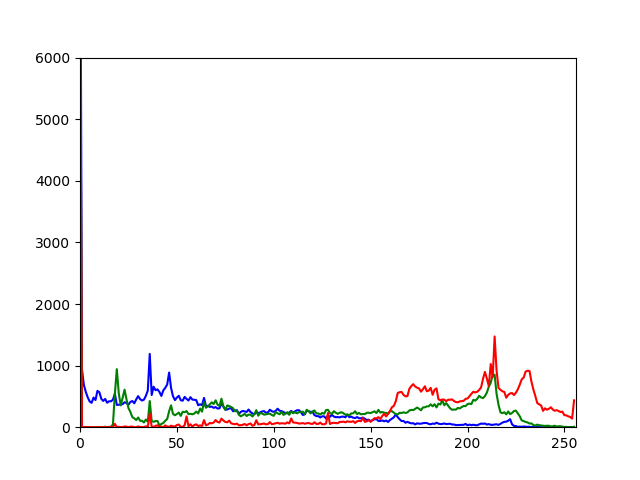
\includegraphics[width=\textwidth]{Sources/Bild3_HA_histo.png}
\end{minipage}
\caption{Histogramm des Segmentierten Objektes aus dem Nahrungsmittel Datensatz. Normalisiert durch den Histogramm Ausgleich}
\label{img:evalHA}
\end{figure}
\newpage
\begin{figure}[htb]
\begin{minipage}[c]{0.2\textwidth}
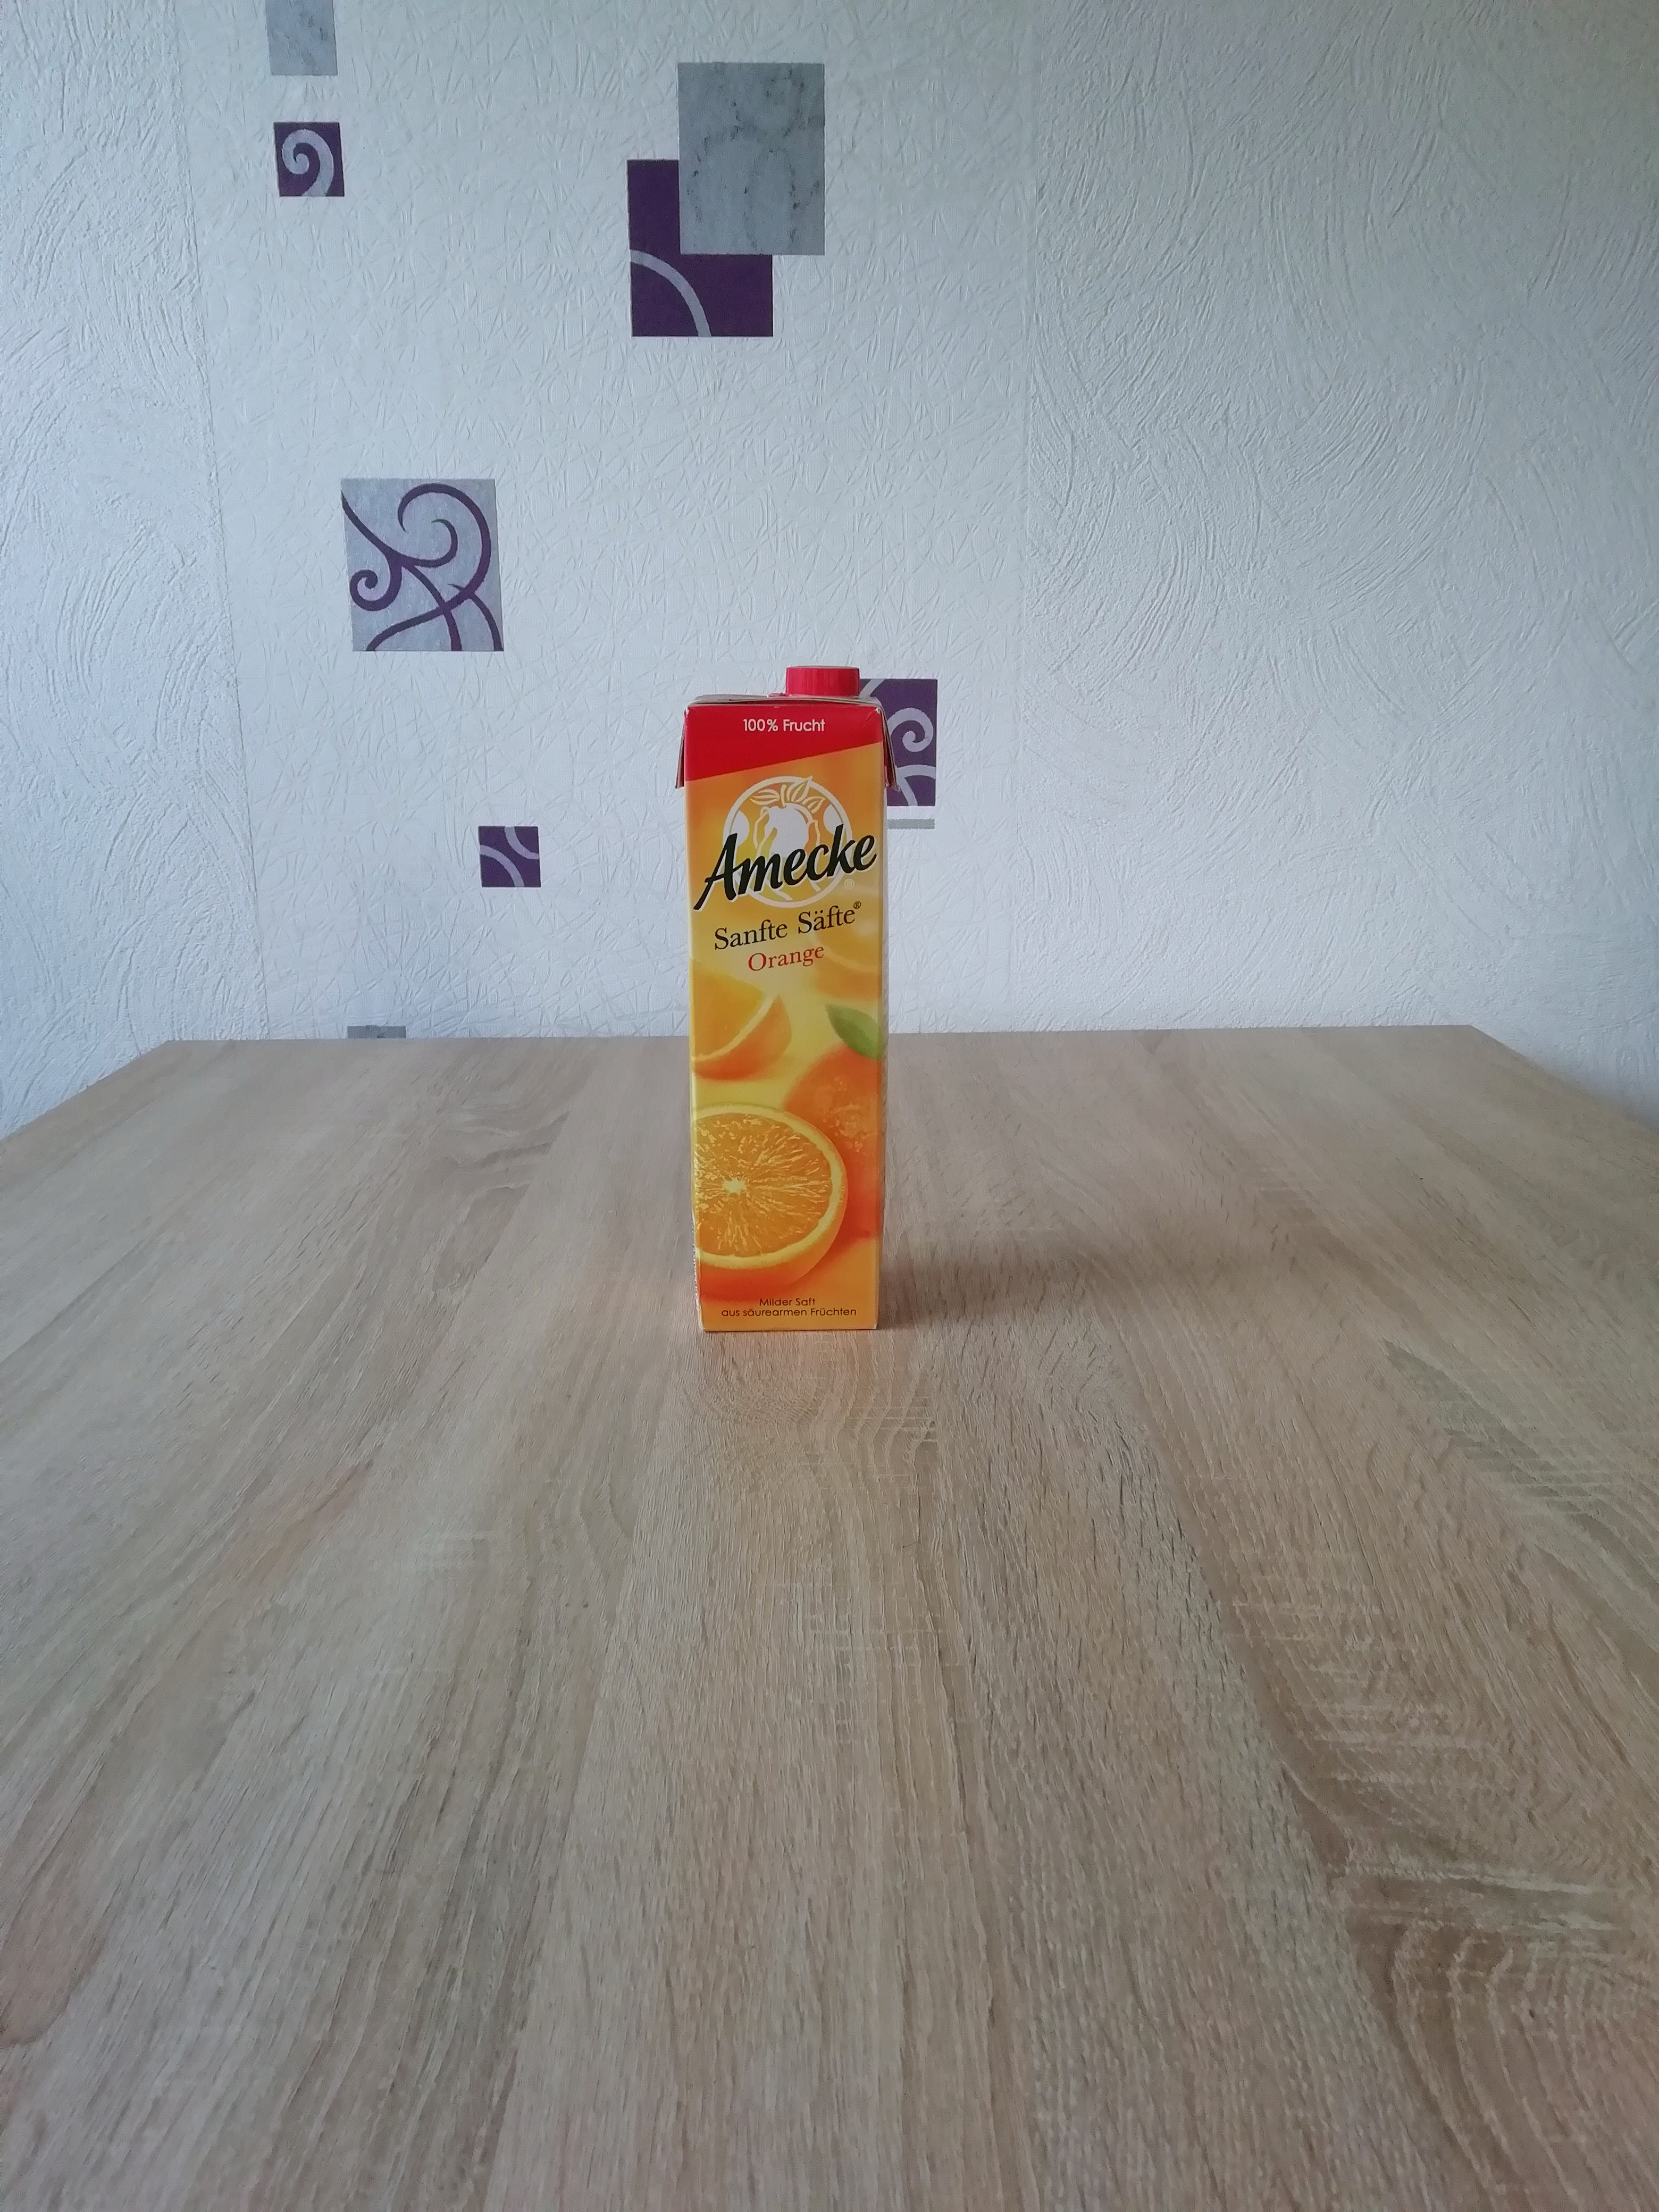
\includegraphics[width=\textwidth]{Sources/Bild1_GW.jpg}
\end{minipage}
\hfill
\begin{minipage}[c]{0.08\textwidth}
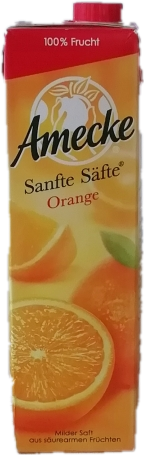
\includegraphics[width=\textwidth]{Sources/Bild1_GW.png}
\end{minipage}
\hfill
\begin{minipage}[c]{0.3\textwidth}
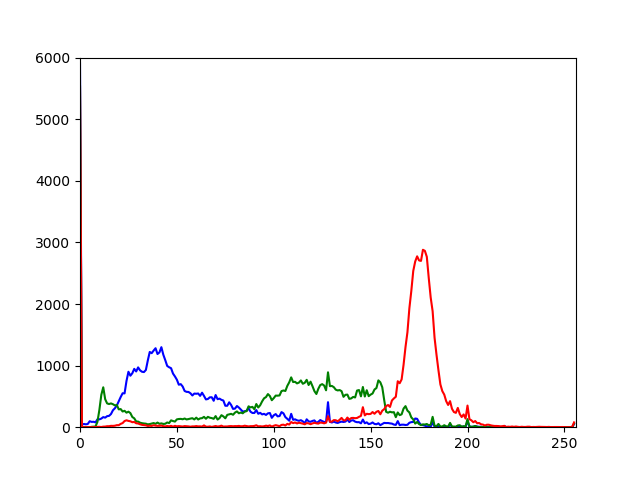
\includegraphics[width=\textwidth]{Sources/Bild1_GW_histo.png}
\end{minipage}
\end{figure}
\begin{figure}[htb]
\begin{minipage}[c]{0.2\textwidth}
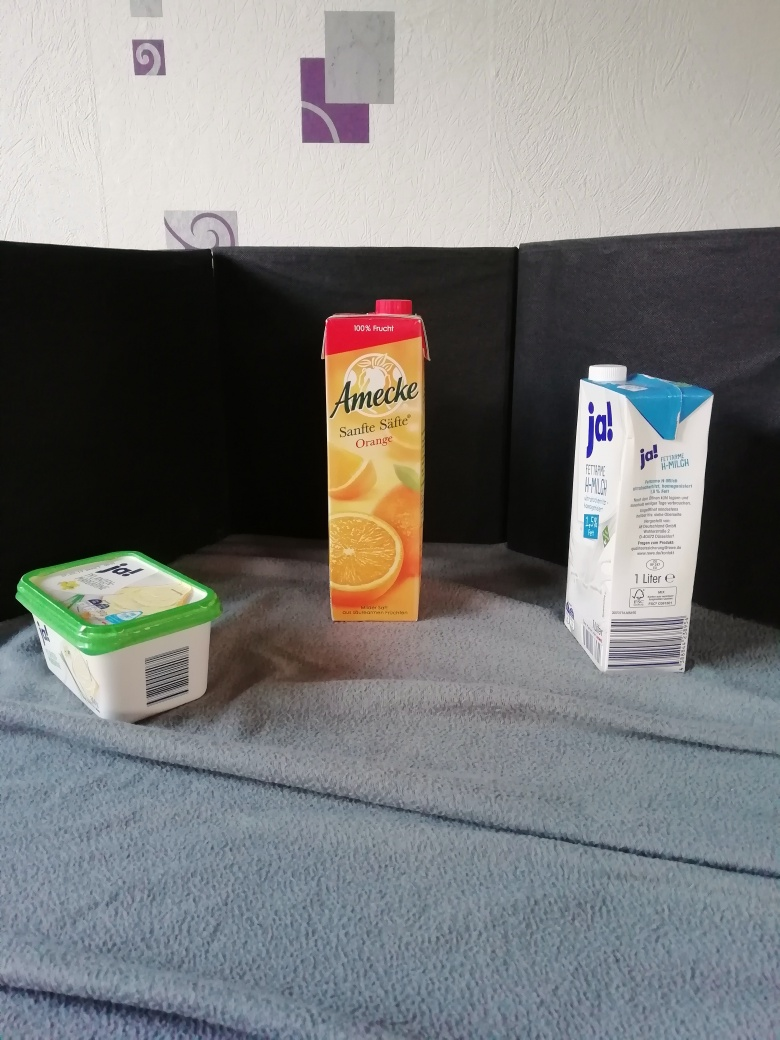
\includegraphics[width=\textwidth]{Sources/Bild2_GW.jpg}
\end{minipage}
\hfill
\begin{minipage}[c]{0.08\textwidth}
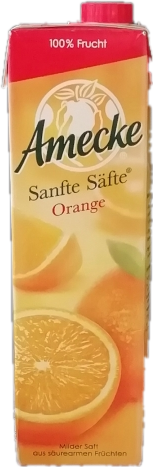
\includegraphics[width=\textwidth]{Sources/Bild2_GW.png}
\end{minipage}
\hfill
\begin{minipage}[c]{0.3\textwidth}
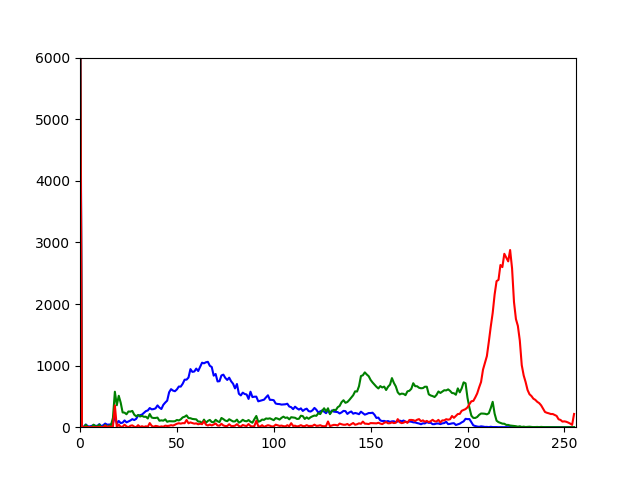
\includegraphics[width=\textwidth]{Sources/Bild2_GW_histo.png}
\end{minipage}
\end{figure}
\begin{figure}[htb]
\begin{minipage}[c]{0.2\textwidth}
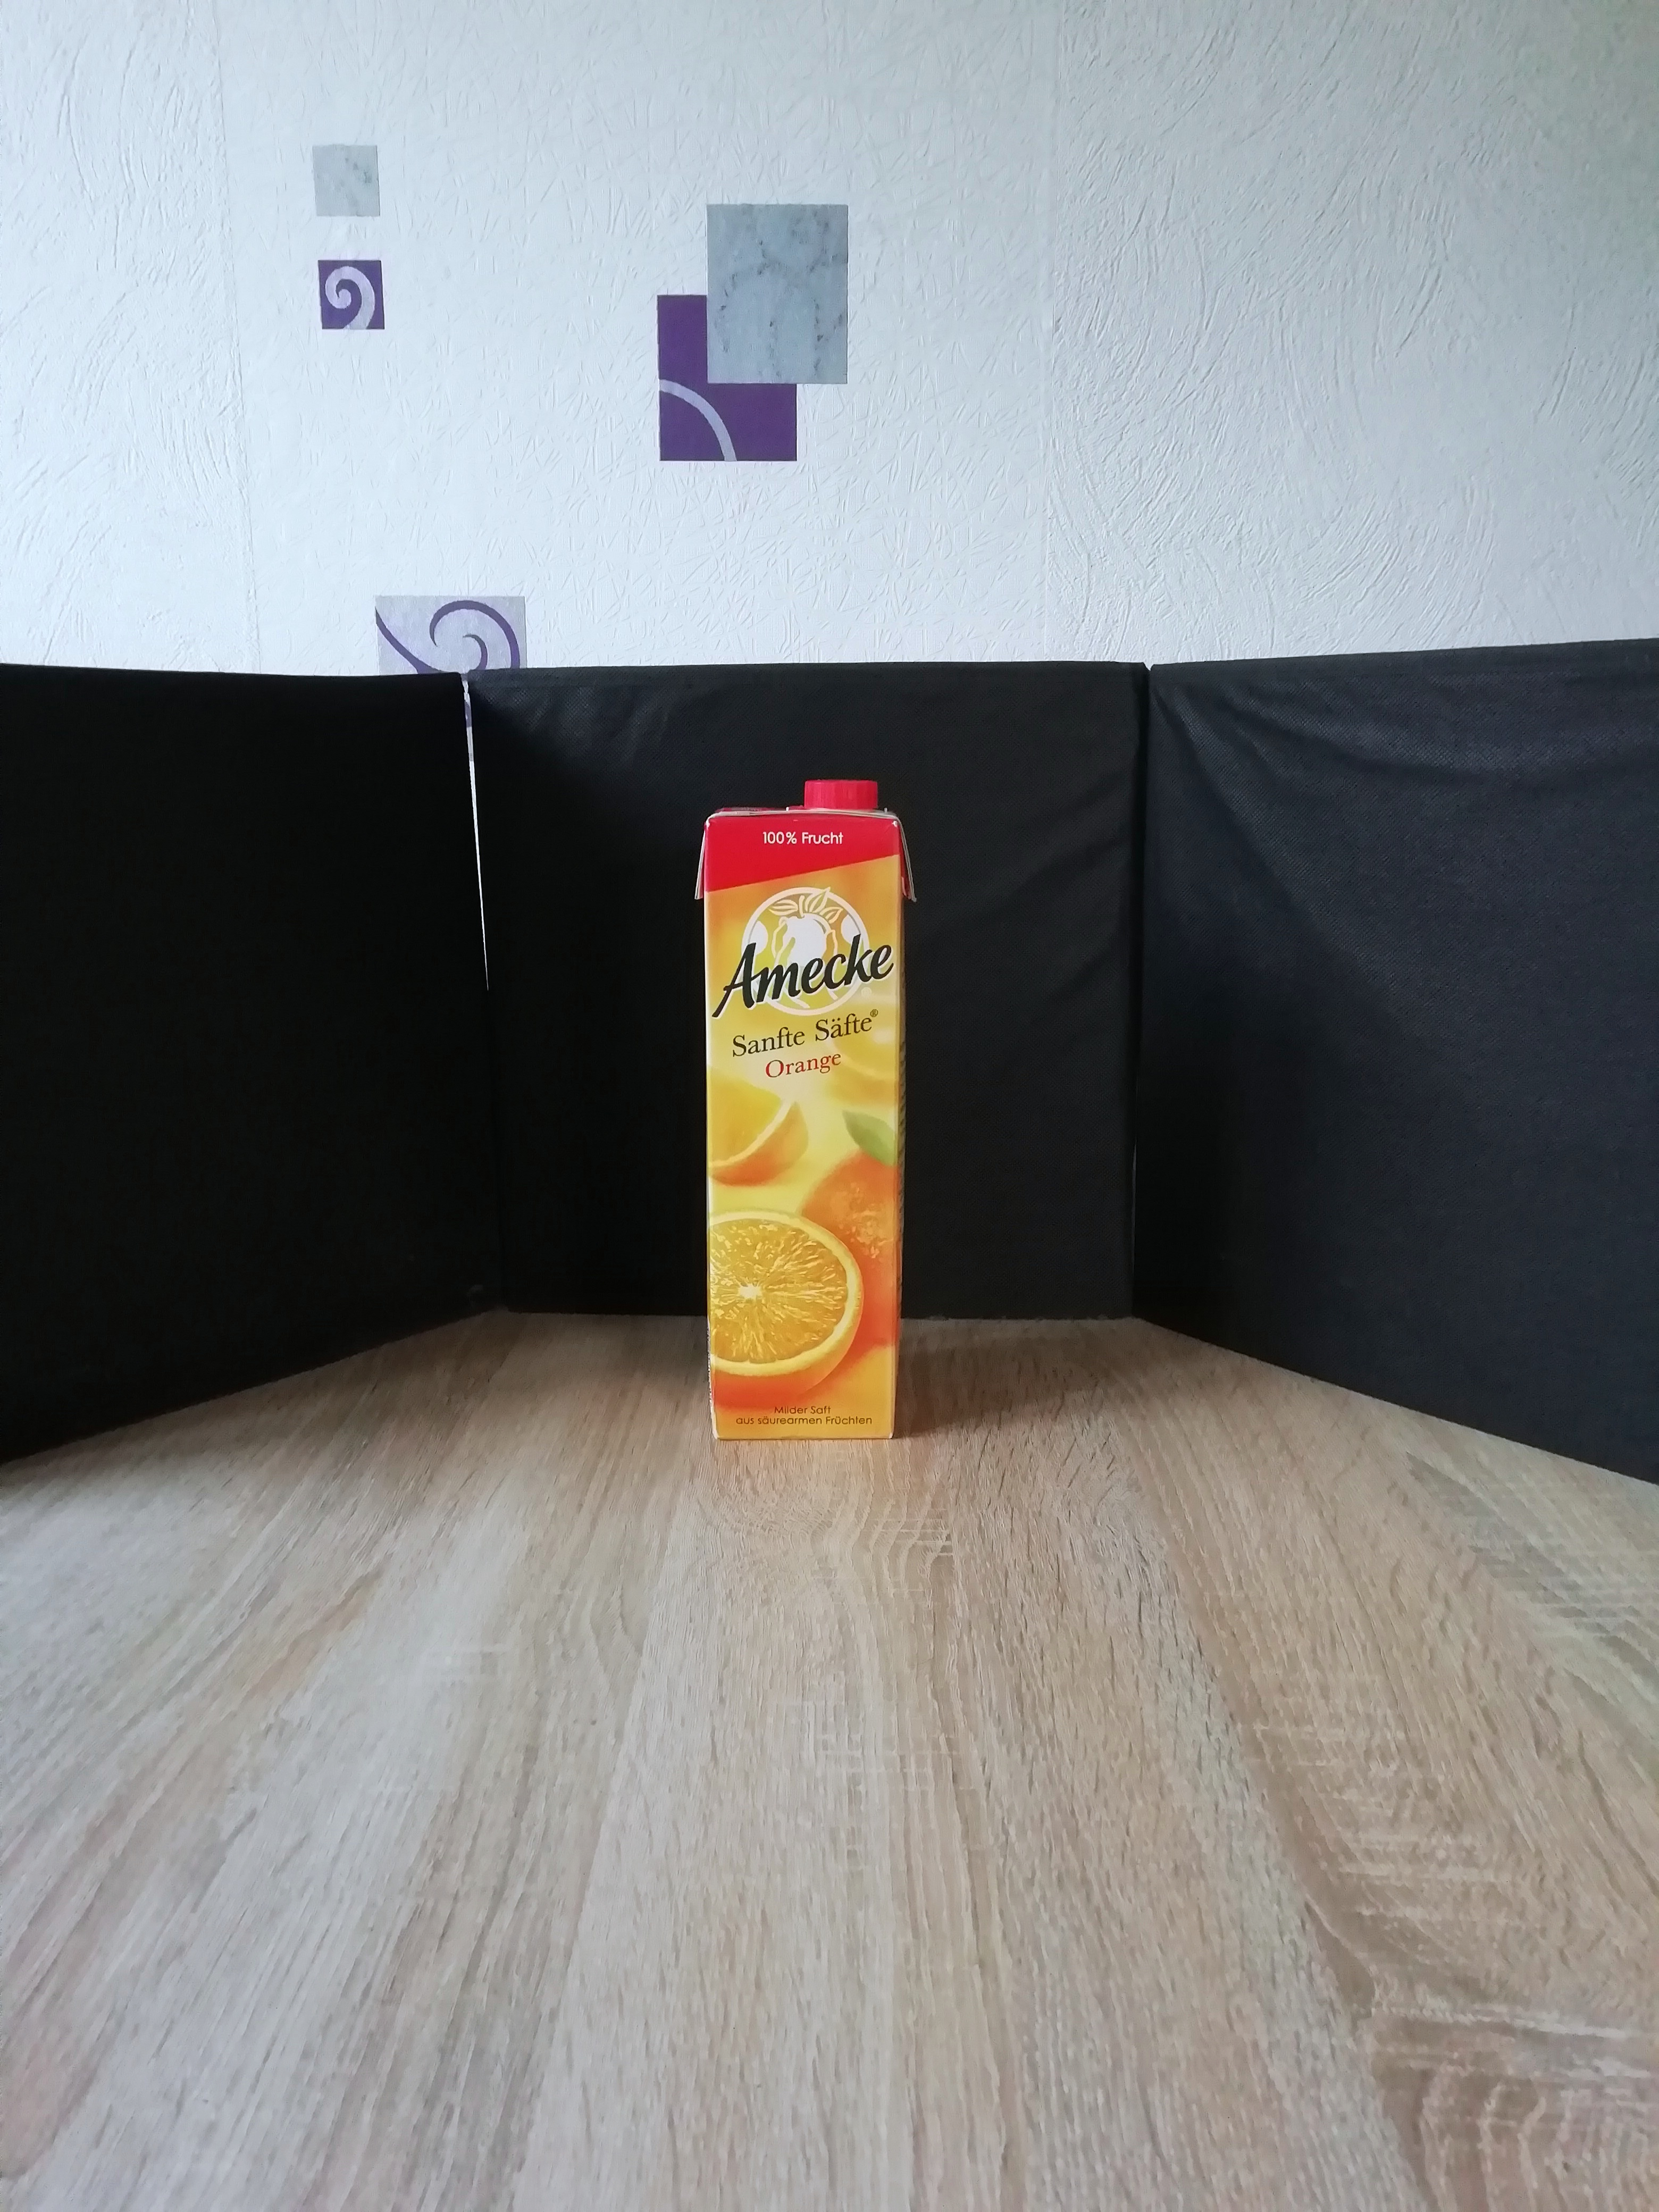
\includegraphics[width=\textwidth]{Sources/Bild3_GW.jpg}
\end{minipage}
\hfill
\begin{minipage}[c]{0.08\textwidth}
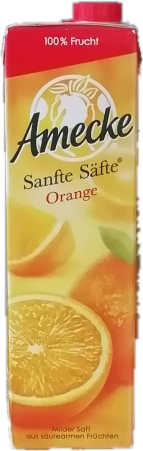
\includegraphics[width=\textwidth]{Sources/Bild3_GW.png}
\end{minipage}
\hfill
\begin{minipage}[c]{0.3\textwidth}
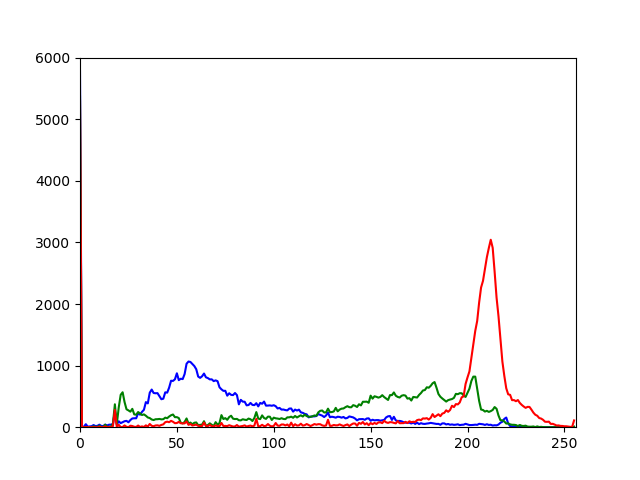
\includegraphics[width=\textwidth]{Sources/Bild3_GW_histo.png}
\end{minipage}
\caption{Histogramm des Segmentierten Objektes aus dem Nahrungsmittel Datensatz. Normalisiert durch den Gray-World Algorithmus}
\label{img:evalGW}
\end{figure}
\newpage
\begin{figure}[htb]
\begin{minipage}[c]{0.2\textwidth}
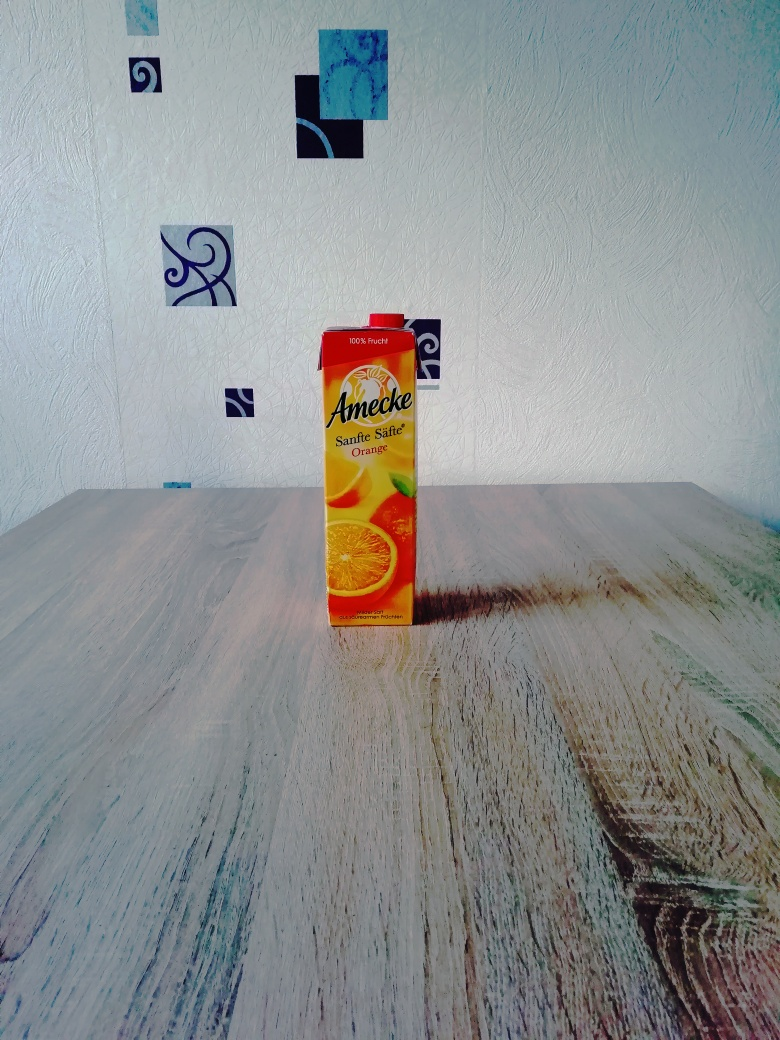
\includegraphics[width=\textwidth]{Sources/Bild1_HS.jpg}
\end{minipage}
\hfill
\begin{minipage}[c]{0.08\textwidth}
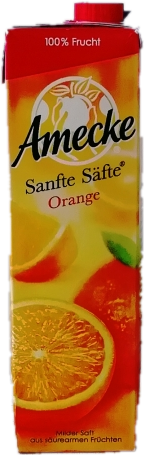
\includegraphics[width=\textwidth]{Sources/Bild1_HS.png}
\end{minipage}
\hfill
\begin{minipage}[c]{0.3\textwidth}
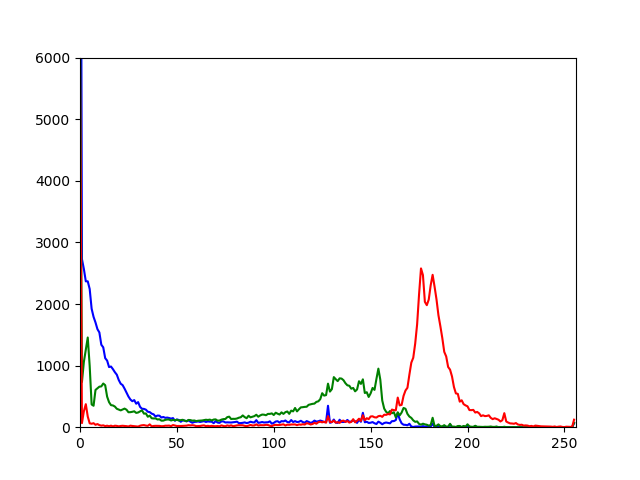
\includegraphics[width=\textwidth]{Sources/Bild1_HS_histo.png}
\end{minipage}
\end{figure}
\begin{figure}[htb]
\begin{minipage}[c]{0.2\textwidth}
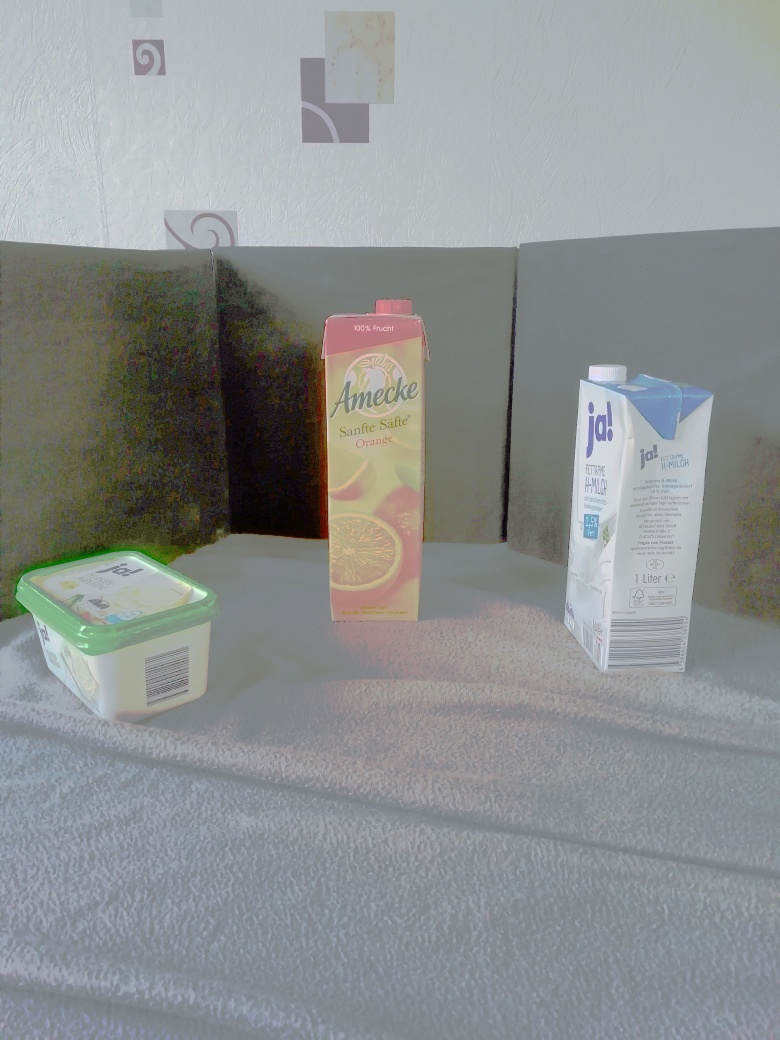
\includegraphics[width=\textwidth]{Sources/Bild2_HS.jpg}
\end{minipage}
\hfill
\begin{minipage}[c]{0.08\textwidth}
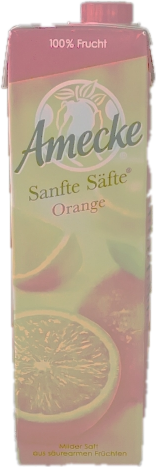
\includegraphics[width=\textwidth]{Sources/Bild2_HS.png}
\end{minipage}
\hfill
\begin{minipage}[c]{0.3\textwidth}
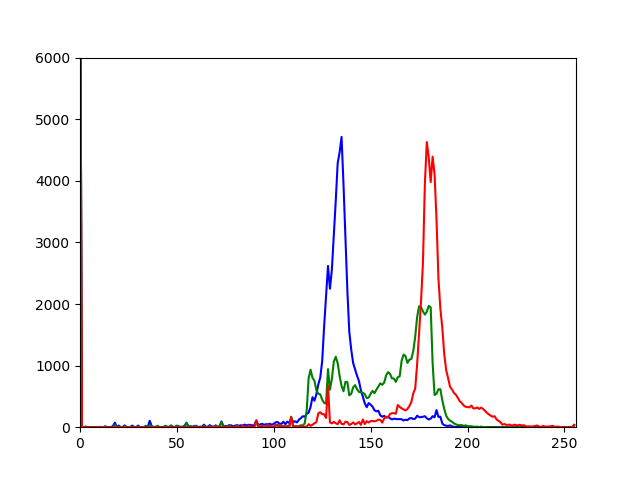
\includegraphics[width=\textwidth]{Sources/Bild2_HS_histo.png}
\end{minipage}
\end{figure}
\begin{figure}[htb]
\begin{minipage}[c]{0.2\textwidth}
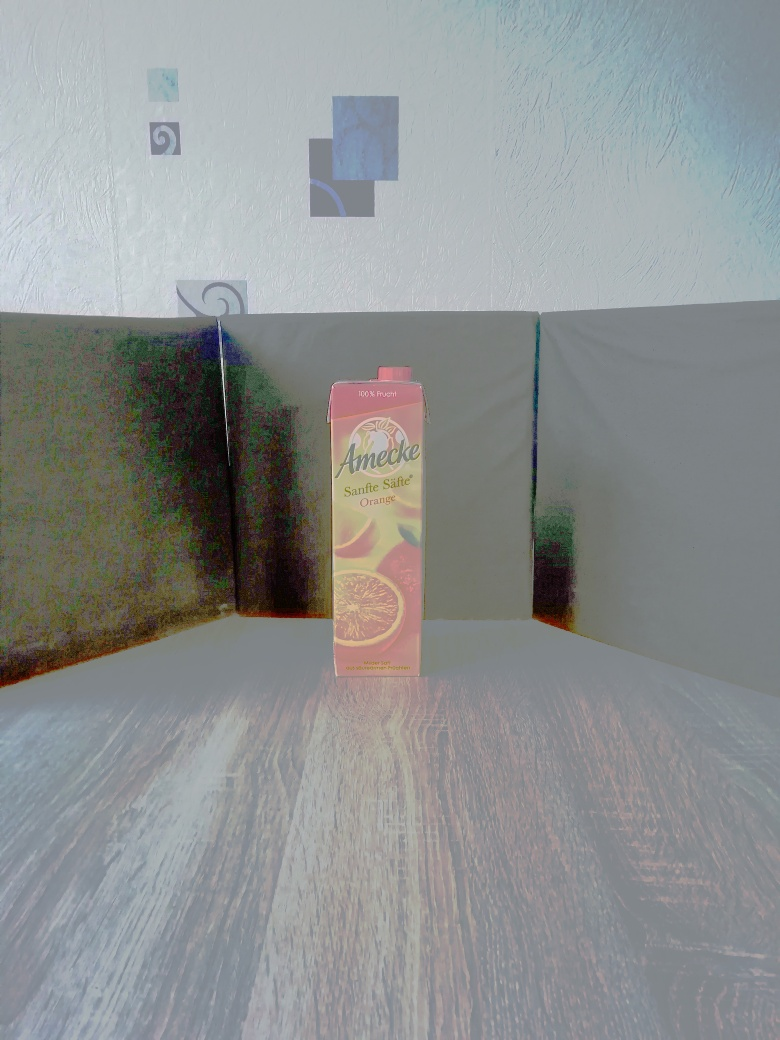
\includegraphics[width=\textwidth]{Sources/Bild3_HS.jpg}
\end{minipage}
\hfill
\begin{minipage}[c]{0.08\textwidth}
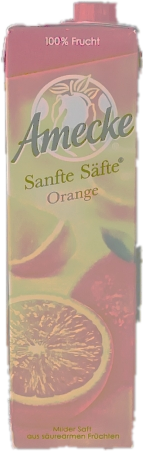
\includegraphics[width=\textwidth]{Sources/Bild3_HS.png}
\end{minipage}
\hfill
\begin{minipage}[c]{0.3\textwidth}
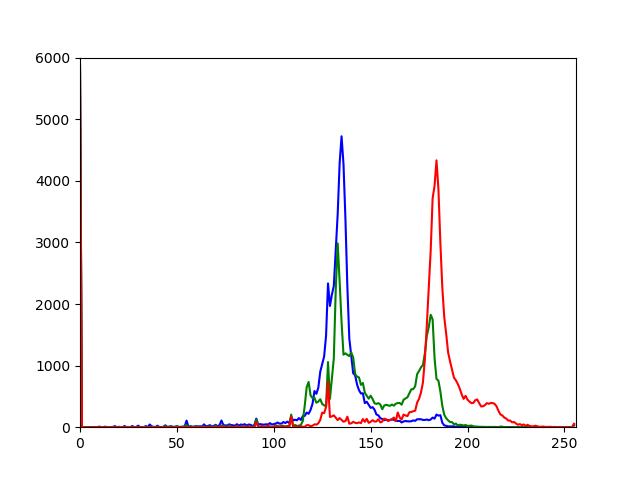
\includegraphics[width=\textwidth]{Sources/Bild3_HS_histo.png}
\end{minipage}
\caption{Histogramm des Segmentierten Objektes aus dem Nahrungsmittel Datensatz. Normalisiert durch die Histogramm Spezifikation}
\label{img:evalHS}
\end{figure}
\newpage
\begin{figure}[htb]
\caption{Helligkeitsverteilung und den Einfluss der Normalisierungs Algorithmen}
\label{img:hellver}
\begin{minipage}[c]{0.4\textwidth}
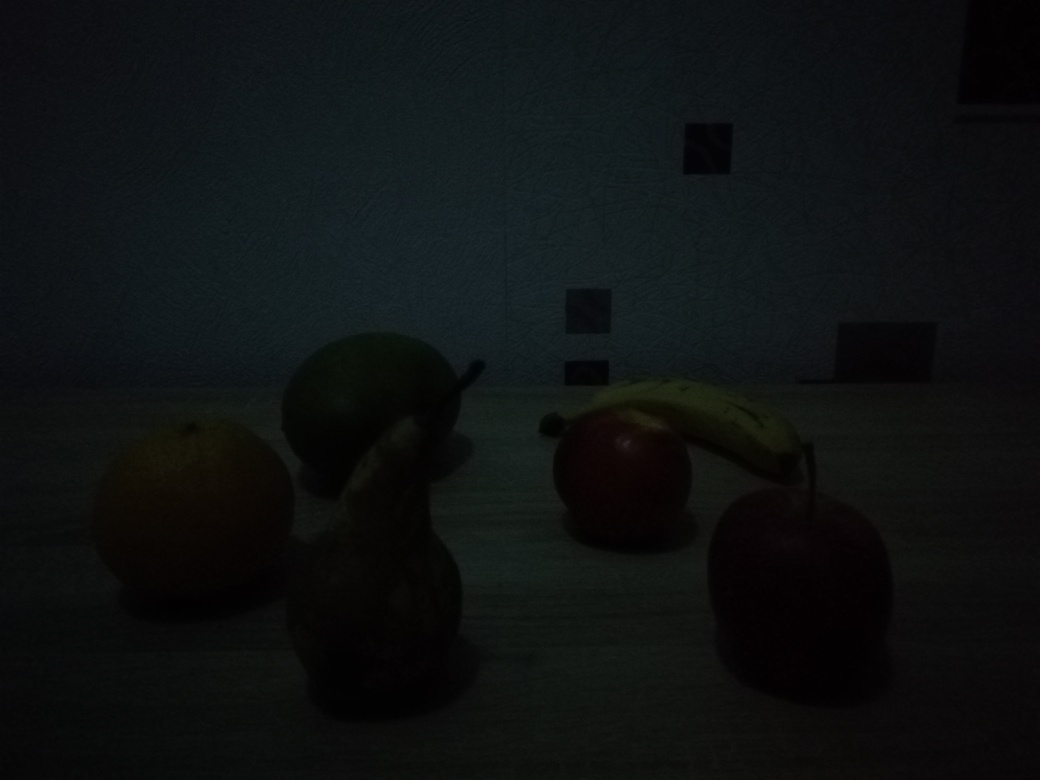
\includegraphics[width=\textwidth]{Sources/Anhang/resize_0250.jpg}
\end{minipage}
\hfill
\begin{minipage}[c]{0.4\textwidth}
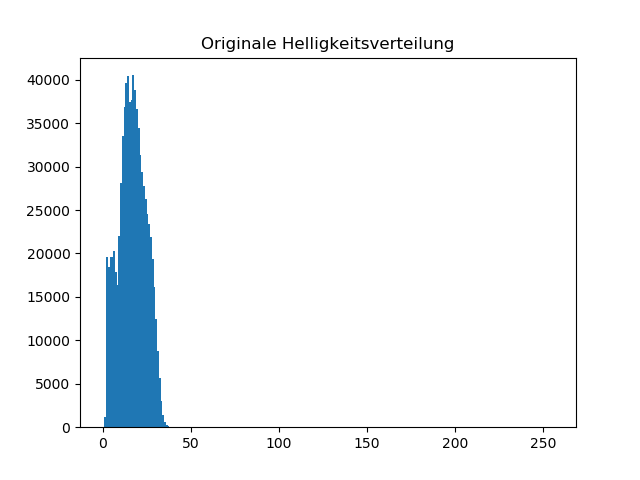
\includegraphics[width=\textwidth]{Sources/Anhang/resize_0250.png}
\end{minipage}
\end{figure}
\begin{figure}[htb]
\begin{minipage}[c]{0.4\textwidth}
\includegraphics[width=\textwidth]{Sources/Anhang/resize_0250_GW.jpg}
\end{minipage}
\hfill
\begin{minipage}[c]{0.4\textwidth}
\includegraphics[width=\textwidth]{Sources/Anhang/resize_0250_GW.png}
\end{minipage}
\end{figure}
\begin{figure}[htb]
\begin{minipage}[c]{0.4\textwidth}
\includegraphics[width=\textwidth]{Sources/Anhang/resize_0250_HA.jpg}
\end{minipage}
\hfill
\begin{minipage}[c]{0.4\textwidth}
\includegraphics[width=\textwidth]{Sources/Anhang/resize_0250_HA.png}
\end{minipage}
\end{figure}
\begin{figure}[htb]
\begin{minipage}[c]{0.4\textwidth}
\includegraphics[width=\textwidth]{Sources/Anhang/resize_0250_HS.jpg}
\end{minipage}
\hfill
\begin{minipage}[c]{0.4\textwidth}
\includegraphics[width=\textwidth]{Sources/Anhang/resize_0250_HS.png}
\end{minipage}
\end{figure}
\newpage
  \section*{Eidesstattliche Erklärung}
Ich versichere, dass ich die Bachelorarbeit selbständig angefertigt und keine anderen als die von mir angegebenen und bei Zitaten kenntlich gemachten Quellen und Hilfsmittel benutzt und die vorliegende Arbeit an keiner anderen Stelle zur Erlangung eines Abschlusses vorgelegt habe.\\\\
 

\vspace{50pt} 
\noindent\rule{5cm}{.4pt}\hfill\rule{5cm}{.4pt}\par 
\noindent Datum, Ort \hfill Unterschrift 
\end{document}

